\PassOptionsToPackage{table}{xcolor}

\documentclass[arabic,a4paper,12pt]{report}
\usepackage{tocloft}
\usepackage[toc,page]{appendix}
  \cftsetindents{table}{0em}{6em}
\cftsetindents{figure}{0em}{6em}  
\renewcommand\cfttabpresnum{Table } % prefix "Table " to table number
\renewcommand\cftfigpresnum{Figure }


\usepackage{microtype}
\usepackage{times}
\usepackage[utf8]{inputenc}
\usepackage{xcolor}

 %%%%********************************************************************
\definecolor{quotemark}{gray}{0.4}
\makeatletter
\def\fquote{%
    \@ifnextchar[{\fquote@i}{\fquote@i[]}%]
           }%
\def\fquote@i[#1]{%
    \def\tempa{#1}%
    \@ifnextchar[{\fquote@ii}{\fquote@ii[]}%]
                 }%
\def\fquote@ii[#1]{%
    \def\tempb{#1}%
    \@ifnextchar[{\fquote@iii}{\fquote@iii[]}%]
                      }%
\def\fquote@iii[#1]{%
    \def\tempc{#1}%
    \vspace{1em}%
    \noindent%
    \begin{list}{}{%
         \setlength{\leftmargin}{0.1\textwidth}%
         \setlength{\rightmargin}{0.1\textwidth}%
                  }%
         \item[]%
         \begin{picture}(0,0)%
         \put(-15,-5){\makebox(0,0){\scalebox{3}{\textcolor{quotemark}{``}}}}%
         \end{picture}%
         \begingroup\itshape}%
 %%%%********************************************************************
 \def\endfquote{%
 \endgroup\par%
 \makebox[0pt][l]{%
 \hspace{0.8\textwidth}%
 \begin{picture}(0,0)(0,0)%
 \put(15,15){\makebox(0,0){%
 \scalebox{3}{\color{quotemark}''}}}%
 \end{picture}}%
 \ifx\tempa\empty%
 \else%
    \ifx\tempc\empty%
       \hfill\rule{100pt}{0.5pt}\\\mbox{}\hfill\tempa,\ \emph{\tempb}%
   \else%
       \hfill\rule{100pt}{0.5pt}\\\mbox{}\hfill\tempa,\ \emph{\tempb},\ \tempc%
   \fi\fi\par%
   \vspace{0.5em}%
 \end{list}%
 }%
 \makeatother
 %%%%********************************************************************


\usepackage{float}
\usepackage{changepage}
\usepackage{multirow}
\usepackage[a4paper]{geometry}
\geometry{left=3.5cm,right=2.5cm,top=3cm,bottom=3cm} % proposition
\usepackage{adjustbox}
\usepackage[utf8]{inputenc}
\usepackage[T1]{fontenc}
\usepackage{enumitem}	
\usepackage{lipsum} %Pour faire des essais
\usepackage{rotating}
\usepackage{tikz}
\usepackage[english,francais]{babel}

\usepackage{lmodern}
\rmfamily \DeclareFontShape{T1}{lmr}{b}{sc}{<->ssub*cmr/bx/sc}{}
\DeclareFontShape{T1}{lmr}{bx}{sc}{<->ssub*cmr/bx/sc}{}

\usepackage{amssymb,amsmath,amsthm,amscd}
\usepackage[all]{xy}
\usepackage{mathrsfs}
\usepackage{appendix}
\usepackage{subfig}

\usepackage{tabularx}
\usepackage{calc}
\usepackage{graphicx}
\usepackage[colorlinks=true,linkcolor=blue]{hyperref}
\usepackage[nottoc]{tocbibind}

\usepackage{color,soul}
%\usepackage[table]{xcolor}



\usepackage[francais]{babel}
\usepackage{amsfonts}
\usepackage{latexsym}
\usepackage{makeidx}
\usepackage{color}
\usepackage{fancyhdr}
\usepackage{stmaryrd}
\usepackage{fancybox}
\pagestyle{fancy}
\fancyhead[L]{}
\usepackage{minitoc}%pour utiliser les mini table of contenent
\usepackage{setspace}
\renewcommand{\baselinestretch}{ 1.3}
 \setcounter{secnumdepth}{4}
\setcounter{tocdepth}{4}
\usepackage[Lenny]{fncychap}
\usepackage{slashbox}
\renewcommand{\theequation}{\thechapter.\arabic{equation}}
\newtheorem*{thm*}{Th�or�me}
\newtheorem*{rem*}{Remarque}
\newtheorem{definition}{Definition}[chapter]
\newtheorem{defn}{D�finition}[chapter]
\newtheorem{theorem}{Theorem}[chapter]
\newtheorem{lemma}{Lemma}[chapter]
\newtheorem{proposition}{Proposition}[chapter]
\newtheorem{corollary}{Corollary}[chapter]
\newtheorem{remark}{Remark}[chapter]
\newtheorem{thm}{Th�or�me}[chapter]
\newtheorem{ep}{Exemple}[chapter]
\newtheorem{lemme}{Lemme}[chapter]
\newtheorem{rem}{Remarque}[chapter]
\newtheorem{pro}{Propri�t�}[chapter]
\newtheorem{prf}{Preuve}[chapter]
\newcommand{\ree}{\mathbb{R}}
\newcommand{\x}{\mathbb{X}}
\newcommand{\z}{\mathbb{Z}}
\newcommand{\s}{\mathcal{S}}
\newcommand{\cc}{\mathcal{C}}
\newcommand{\f}{\mathcal{F}}
\newcommand{\g}{\mathcal{G}}
\newcommand{\m}{\mathbb{M}}
\definecolor{arylideyellow}{rgb}{0.91, 0.84, 0.42}
\newcommand{\listappendicesname}{Appendices}

%==========================================================================================================
% =========================== Commandes diverses ===============================

%\input{macros}
%\input{macrosmath}

% =========================== Info du document =================================

\title{Du bouturage des gard�nias}


\begin{document}

\selectlanguage{french}

%\addtocounter{page}{-1}
%\include{pagedegarde}
%\pdfbookmark[0]{Page de garde}{garde}
% La commande pdfbookmark permet � hyperref d'ajouter la page de garde dans le
% menu du fichier compil� (dvi, pdf)

\thispagestyle{empty}
% pour ne pas avoir de num�ro de page sur la page de garde -- le compteur de
% page est cependant � 1, c'est-�-dire que la num�rotation commence � partir
% de la page de garde

\begin{center}
  \begin{tabularx}{\textwidth}{m{1.5cm}Xm{1.5cm}X}
    
\includegraphics[width = 3cm]{Figures/logo2bis}
    & \begin{center}{\textbf{ Université Hassan Premier}\\
{\textbf{Ecole Nationale des Sciences Appliquées -Khouribga-}}}

 \vspace{\stretch{2}}% Permet de cr�er un espace vertical de longueur variable (\stretch) et de "poids" 2

\end{center}
       & 
\includegraphics[width =3cm]{Figures/logo1bis}\\
  \end{tabularx}
\end{center}
%%\hspace{\stretch{2}}\boxed{N� d'ordre: 05/2018}
\begin{center}



\vspace{\stretch{1}} \textbf{Projet de fin d'études} 


En vue de l'obtention du diplôme 

\vspace{\stretch{2}}
{\Huge \textsc{INGENIEUR D'ETAT}}\\
\textbf{Filiére : Génie Informatique }

\vspace{\stretch{2}}
\textbf{Présenté par}\\
\textbf{Mohammed Amine MAGHOUS }

\vspace{\stretch{2}}

\hrule \vspace{\stretch{1}} {\LARGE \textbf{ Extension des fonctionnalités d'un système distribué de traitement de graphes PGX.D et la mesure de sa performance avec TPC-H }} \vspace{\stretch{1}} \hrule
\vspace{\stretch{1}}


% \vspace{\stretch{2}}

% Soutenu le 12 Juillet 2018, devant le jury :

% \vspace{\stretch{2}} {\Large
% \begin{tabular}{lll}
% \small M. Omar EL BANNAY &\small ENSA Khouribga  &\small Président\\
% \small M. Mostafa SAADI&\small ENSA Khouribga   &\small Examinateur\\
% \small Mme. Meriem MANDAR &\small ENSA Khouribga  &\small Encadrante Interne\\
% \small M. Abdelfettah CHEFFI &\small Hightech Payment Systems  &\small Encadrant Externe\\
% \end{tabular}
% }

\end{center}

\cleardoublepage % pour laisser une page blanche au verso de la page de garde


\newpage
\newpage
  \pdfbookmark[0]{Page de garde}{garde}
% La commande pdfbookmark permet � hyperref d'ajouter la page de garde dans le
% menu du fichier compil� (dvi, pdf)

\thispagestyle{empty}
% pour ne pas avoir de num�ro de page sur la page de garde -- le compteur de
% page est cependant � 1, c'est-�-dire que la num�rotation commence � partir
% de la page de garde

\begin{center}
  \begin{tabularx}{\textwidth}{m{1.5cm}Xm{1.5cm}X}
    
\includegraphics[width = 3cm]{Figures/logo2bis}
    & \begin{center}{\textbf{ Université Hassan Premier}\\
{\textbf{Ecole Nationale des Sciences Appliquées -Khouribga-}}}

 \vspace{\stretch{2}}% Permet de cr�er un espace vertical de longueur variable (\stretch) et de "poids" 2

\end{center}
       & 
\includegraphics[width =3cm]{Figures/logo1bis}\\
  \end{tabularx}
\end{center}
%%\hspace{\stretch{2}}\boxed{N� d'ordre: 05/2018}
\begin{center}



\vspace{\stretch{1}} \textbf{Projet de fin d'études} 


En vue de l'obtention du diplôme 

\vspace{\stretch{2}}
{\Huge \textsc{INGENIEUR D'ETAT}}\\
\textbf{Filiére : Génie Informatique }

\vspace{\stretch{2}}
\textbf{Présenté par}\\
\textbf{Mohammed Amine MAGHOUS }

\vspace{\stretch{2}}

\hrule \vspace{\stretch{1}} {\LARGE \textbf{ Extension des fonctionnalités d'un système distribué de traitement de graphes PGX.D et la mesure de sa performance avec TPC-H }} \vspace{\stretch{1}} \hrule
\vspace{\stretch{1}}


% \vspace{\stretch{2}}

% Soutenu le 12 Juillet 2018, devant le jury :

% \vspace{\stretch{2}} {\Large
% \begin{tabular}{lll}
% \small M. Omar EL BANNAY &\small ENSA Khouribga  &\small Président\\
% \small M. Mostafa SAADI&\small ENSA Khouribga   &\small Examinateur\\
% \small Mme. Meriem MANDAR &\small ENSA Khouribga  &\small Encadrante Interne\\
% \small M. Abdelfettah CHEFFI &\small Hightech Payment Systems  &\small Encadrant Externe\\
% \end{tabular}
% }

\end{center}

\cleardoublepage % pour laisser une page blanche au verso de la page de garde


\newpage

\chapter*{Dédicace}

\begin{fquote}
\begin{center}
\large{
Je dédie ce travail:\\[12pt]
\uppercase{à} ma chère mère et à mon cher père qui n'ont jamais cessé de me supporter, me soutenir et m'encourager durant mes années d'études.
Qu'ils trouvent ici le témoignage de ma profonde gratitude et reconnaissance.
\uppercase{à} mes frères, mes grands-parents et ma famille qui me donnent de l'amour et de la vivacité.
\uppercase{à} tous ceux qui m'ont aidé - de près ou de loin - et ceux qui ont partagé avec moi les moments d'émotion lors de la réalisation de ce travail et qui m'ont chaleureusement supporté et encouragé tout au long de mon parcours.
\uppercase{à} tous mes amis qui m'ont toujours encouragé, et à qui je souhaite plus de succès.\\
Merci!
}
\end{center}
\bigskip
\medskip
\end{fquote}

\begin{adjustwidth}{2cm}{1cm}
\hspace*{\fill} \textbf{\textit{\large{- Mohammed Amine Maghous}}}
\end{adjustwidth}

\clearpage
\newpage
  \chapter*{Remerciements}
Avant de présenter mon travail, je voudrais exprimer ma grande reconnaissance à ceux qui m'ont soutenu,
de près ou de loin. Je souhaite qu'ils trouvent ici, collectivement et individuellement,
l'expression de toute ma gratitude et de mon appréciation. Je tiens à exprimer mes remerciements et ma gratitude
à M. KOUPY Petr, M. TRIGONAKIS Vasileios et M. IORGULESCU Calin, ainsi qu'à toute l'équipe de PGX Distributed,
pour l'expérience enrichissante et intéressante qu'ils m'ont fait vivre pendant la durée du stage,
pour tous les conseils et informations qu'ils m'ont donnés et pour le temps qu'ils ont consacré à la supervision
et au suivi de ce travail. Je tiens également à remercier mes professeurs superviseurs M. SAADI Mohamed et
M. GHERABI Noureddine, malgré leurs multiples responsabilités, qui nous ont assuré le suivi de ce projet.
Je tiens également à exprimer mes plus sincères remerciements à l'ensemble du personnel administratif et enseignant
de l'ENSA Khouribga, pour avoir porté un vif intérêt à notre formation, et pour y avoir apporté attention et énergie,
et ce, dans un environnement agréable et respectueux. Que les membres du jury trouvent dans cet ouvrage l'expression de ma gratitude pour
l'honneur qu'ils me font en prenant le temps de lire et d'évaluer cet ouvrage.
%%%%%%%%%%%%%%%%%%%%%%%%%%%%%%%%%%%%%%%%%%%%%%%%%%%%%%%%%%%%%%%%%%%%%%%%%%%%%%%%%%%%%%%%%%%%\chapter*{Remerciements}
Avant de présenter mon travail, je voudrais exprimer ma grande reconnaissance à ceux qui m'ont soutenu,
de près ou de loin. Je souhaite qu'ils trouvent ici, collectivement et individuellement,
l'expression de toute ma gratitude et de mon appréciation. Je tiens à exprimer mes remerciements et ma gratitude
à M. KOUPY Petr, M. TRIGONAKIS Vasileios et M. IORGULESCU Calin, ainsi qu'à toute l'équipe de PGX Distributed,
pour l'expérience enrichissante et intéressante qu'ils m'ont fait vivre pendant la durée du stage,
pour tous les conseils et informations qu'ils m'ont donnés et pour le temps qu'ils ont consacré à la supervision
et au suivi de ce travail. Je tiens également à remercier mes professeurs superviseurs M. SAADI Mohamed et
M. GHERABI Noureddine, malgré leurs multiples responsabilités, qui nous ont assuré le suivi de ce projet.
Je tiens également à exprimer mes plus sincères remerciements à l'ensemble du personnel administratif et enseignant
de l'ENSA Khouribga, pour avoir porté un vif intérêt à notre formation, et pour y avoir apporté attention et énergie,
et ce, dans un environnement agréable et respectueux. Que les membres du jury trouvent dans cet ouvrage l'expression de ma gratitude pour
l'honneur qu'ils me font en prenant le temps de lire et d'évaluer cet ouvrage.


%\newpage
\pdfbookmark[0]{Résumé}{resume}


\chapter*{Résumé}
De nos jours, la plupart des données sont organisées sous forme de tableaux. Par exemple, si l'on considère les applications bancaires, la manière typique d'organiser la plupart des données est celle des tableaux où les clients ont des comptes, les comptes ont des transactions, et les transactions se font entre les comptes (un chiffre ici), ce type d'organisation a son application là où elle excelle et c'est pourquoi les bases de données relationnelles existent depuis les années 80. Cependant, une autre façon de voir les choses est que les clients font des transactions avec d'autres clients via leurs comptes et que les comptes sont reliés entre eux par des transactions, ce qui donne un graphe, et cette façon de voir permet aux gens de poser des questions plus intéressantes qui résident dans ces connexions, prenez par exemple une carte mentale, un des outils utiles utilisés lorsque l'on est bloqué ou que l'on a besoin d'expliquer une idée de façon intuitive. 
\\ \\
De nombreux outils ont été créés pour tirer le meilleur parti de ces nouvelles façons de représenter les données, partant des bases de données de graphes comme Neo4j, jusqu'aux outils de traitement de graphes comme PGX.D, celui qui sera abordé dans ce rapport, qui est parmi les engins de traitement de graphes les plus avancés dans ce domaine. PGX.D brille particulièrement lorsqu'il s'agit de données qui ne peuvent pas être stockées dans la mémoire d'une seule machine, ou de données dont la taille peut augmenter considérablement avec le temps, comme les graphes sociaux de Facebook et Twitter par exemple. Dans ce rapport, je présenterai ma contribution à l'effort continu d'extension des capacités de PGX.D, allant du filtrage des graphes à l'analyse des performances avec TCP-H et enfin à la prise en charge des valeurs nulles dans les "frames".
\\ \\

\noindent\textbf{Mots clés :} Filtrage des graphes, TPC-H benchmarking, NULL values

\newpage
\chapter*{Abstract}
Nowadays most data is organized in the form of tables, for instance if we look at banking application the typical way of organizing most data is tables where customers have accounts, accounts have transactions, and transactions are between accounts (a figure here), this type of organizations have their application where they excel at and that’s why relational databases exist since the 80’s. However, a different way to looking at it, is that customers are transacting with other customers via their accounts and the accounts are connected via transactions, which results in a graph, and looking at this way allows people to ask more interesting questions that reside into those relationships, take as an example a mind map one of the useful tools used when one is stuck or need to explain an idea intuitively. 
\\ \\
A lot of tools have been created to take the most from these new ways of representing data from graph databases, to graph processing tools like PGX.D, the one we will discuss in this report, which is among the most advanced graph in this field. PGX.D shines especially when it comes to data that cannot fit into the memory of a single machine, or data that can grow significantly in size by time like, Facebook, and Twitter social graphs for instance. In this report I will present my contribution to the ongoing effort of extending the capabilities of PGX.D, from graph filtering to benchmarking and finally null value support in frames
\\ \\ \\ \\
\noindent\textbf{Keywords :} Graph filtering, TPC-H benchmarking, NULL values

\newpage





\chapter*{Liste des abréviations}
\addcontentsline{toc}{chapter}{Liste des abréviations}

\renewcommand{\arraystretch}{1.15}
\begin{table}[ht]
\begin{center}
\rowcolors{1}{}{lightgray}
\begin{tabular}{p{4cm}p{9cm}}
  \hline
Acronyme & Signification \\
  \hline
API & Application Programming Interface \\
BD & Base de données \\
CSS & Cascading Style Sheet \\
DAO & Data Access Object \\
DP & Directeur de Projet \\
FDT & Feuille De Temps \\
GAB & Guichet Automatique de Banque \\
HPS & Hightech Payment Systems \\
HTML & HyperText Markup Language \\
HTTP & Hypertext Transfer Protocol \\
IDE & Integrated Development Environment \\
IHM & Interface Homme-Machine\\
Java EE & Java Entreprise Edition \\
JDBC & Java DataBase Connectivity \\
JSON & JavaScript Object Notation \\
MVC & Model View Controller \\
MVVM & Model View ViewModel \\
PMO & Project Manager Officer \\
REST & Representational State Transfer \\
RH & Ressource Humaine \\
SGBD & Systèmes de Gestion de Base de Données \\
SQL & Structered Query Language \\
TDB & Tableau de bord \\
TPE & Terminal de Paiement Electronique \\
UML & Unified Modeling Language \\
XP & Extreme Programming \\
   \hline
\end{tabular}

\end{center}
\end{table}
\renewcommand{\arraystretch}{1}

%%%%%%%%%%%%%%%%%%%%%%%%%%%%%%%%%%%%%%%%%%%%%%%%%%%%%%%%%%%%%%%%%%%%%%%%%%%%%%%%%%%%%%%%%%%%%%%%%%%%�\include{r�sum�}

\setcounter{tocdepth}{2} \pdfbookmark[0]{Table des
mati�res}{tablematieres}
%%%%%%%%%%%%%%%%%%%%%%%%%%%%%%%%%%%%%%%%%%%%%%%%%%%%%%%%%%%%%%%%%%%%%%%%%%%%%%%%%%%%%%%%%%%%%�\include{pr�sentation}


\tableofcontents
\newpage
% list of tables
\listoftables

% list of figures
\listoffigures


\chapter*{Introduction Générale}
\addcontentsline{toc}{chapter}{Introduction Générale}
Au cours des dernières décennies, nous avons assisté à une nouvelle tendance dans l'histoire de l'informatique : les chercheurs déplacent progressivement leur analyse de l'étude de l'individu vers celle du collectif. Nous pouvons percevoir ce changement dans de nombreux domaines. En combinant des données provenant de sources multiples, les chercheurs ont commencé à observer et à analyser le comportement collectif des foules [a.5], les changements physiques de notre environnement, les interactions sociales et monétaires des populations, la propagation des maladies et la consommation d'énergie dans les villes, entre autres.\\

Chacun de ces domaines présente des caractéristiques uniques. Pourtant, dans de nombreuses applications, notamment la détection, [b.3] la finance, l'épidémiologie et la biologie, on trouve une approche sous-jacente commune : la modélisation des dépendances d'entités interconnectées sous forme de graphes.\\

Pour tirer parti de cette nouvelle façon de représenter les données, de nombreux outils et techniques ont vu le jour. Les bases de données de graphes comme Neo4j, sont optimisées pour des requêtes avec lesquelles la base de données relationnelle peut facilement souffrir, ces requêtes contiennent généralement beaucoup de jointures, et même si les professionnels des bases de données relationnelles ont essayé pendant des décennies d'optimiser cela, le nombre de résultats intermédiaires peut croître exponentiellement en taille, ce qui peut parfois même remplir toute la mémoire disponible sur le disque.\\

Généralement, ces outils proposent leur propre langage de requête SQL, même si ces langages ont récemment convergé vers une syntaxe similaire, et donc une requête de sur un graphe, habituellement ressemblera à cela dans beaucoup de ces systèmes :\\
\begin{figure}[H]  
 \centering
    
\includegraphics[width=1\textwidth]{exmp_pgql.PNG}
\end{figure}
Si nous supposons qu'il s'agit d'un site de commerce électronique, cette requête sélectionnera le nom de toutes les personnes travaillant dans le département informatique.\\
La même requête en SQL deviendra moins intuitive et ressemblera à ceci :
\begin{figure}[H]  
 \centering
    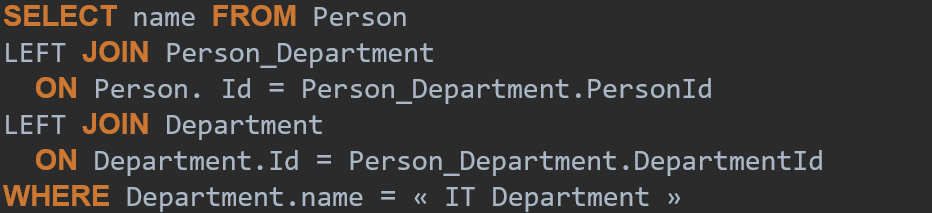
\includegraphics[width=1\textwidth]{exmp_sql.PNG}
\end{figure}

Le traitement de graphes gigantesques, des graphes pouvant atteindre des dizaines de téraoctets, présente ses propres défis. La recherche d’une faible latence nécessitera le chargement du graphe en mémoire pour le traiter, car la vitesse du disque est encore aujourd’hui très lente par rapport à la RAM. Peu de machines peuvent avoir assez de mémoire pour ce genre de charge de travail, et même si une machine avait autant de mémoire, que se passera-t-il si la taille augmente très rapidement, que la mise à l’échelle du nœud du calcule sera insuffisante ? Le système ne pourra pas contenir toutes ces données, et c’est là que PGX.D [a.2], [a.3] vient à la rescousse, puisque ce système est un système distribué, la mise à l’échelle par l’ajout d’autres nœuds serait naturelle et peut être moins coûteuse puisque vous pouvez n’utiliser que les machines que vous jugez nécessaires.\\
Dans ce rapport, je présenterai ma contribution au projet PGX.D ou je me concentrerai sur les points suivants :\\
\begin{itemize}[label=\textbullet]
\item Présentation de l’organisme d’accueil, et le projet PGX.
\item Présenter et expliquer des notions fondamentales pour comprendre ce système.
\item L’extension du support de filtrage, en ajoutant la possibilité de créer un sous-graph à partir d’une collection de sommets/bords ainsi que l’opération inverse.
\item Ajout du support aux propriétés NULL dans les « frames ».
\item Benchmarking avec TPC-H.
\end{itemize}

Des annexes seront proposées en fin du rapport pour développer quelques aspects clés qui n’ont pas été approfondis dans les différentes parties.

\chapter{Contexte général du projet}

\section{Présentation de l’organisme d’accueil}
\subsection{Présentation de ORACLE}
Oracle Corporation est une multinationale américaine de technologie informatique spécialisée principalement dans le développement et la commercialisation de logiciels et de technologies de bases de données, de systèmes "cloud engineered" et de logiciels d'entreprise - en particulier ses propres marques de systèmes de gestion de bases de données. Son siège social est situé en Redwood City, United States [b.13].

\subsection{Oracle en nombres}
\begin{table}[h!]  
  \centering
    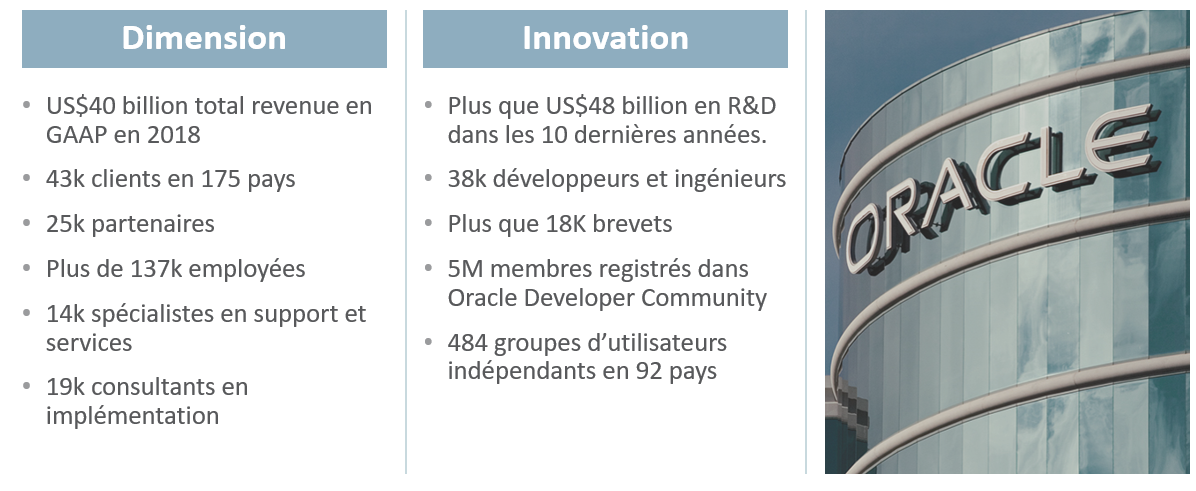
\includegraphics[width=0.8\textwidth]{chapitre1/Figures/OracleNumbers.PNG}
  \caption{Oracle, dimension et innovation}
\end{table}

\subsection{Leadership d'Oracle}
Oracle est considéré leader mondiale dans ces domaines :
\begin{table}[h!]  
  \centering
    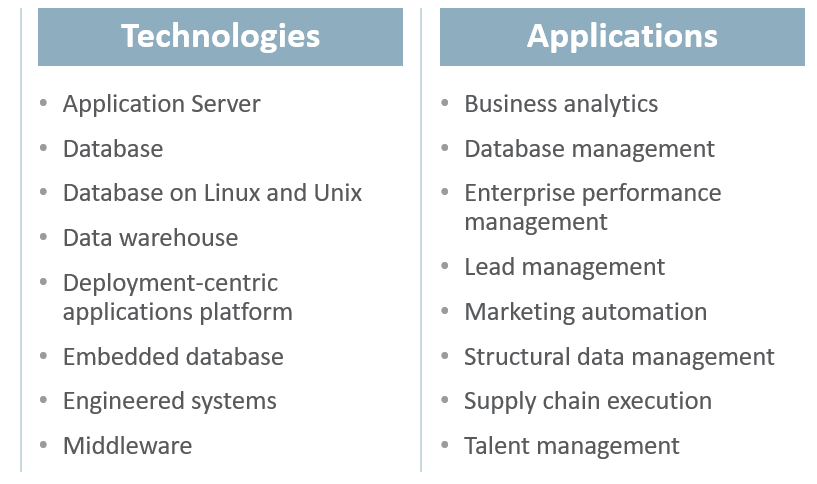
\includegraphics[width=0.8\textwidth]{chapitre1/Figures/OrcaleTechnos.PNG}
  \caption{Oracle, leader en plusieurs technologies et services}
\end{table}

\subsection{Clients Oracle}
La majorité des entreprises leader dans leur domaine, utilise des produits ou services d’Oracle.
\begin{figure}[h!]  
  \centering
    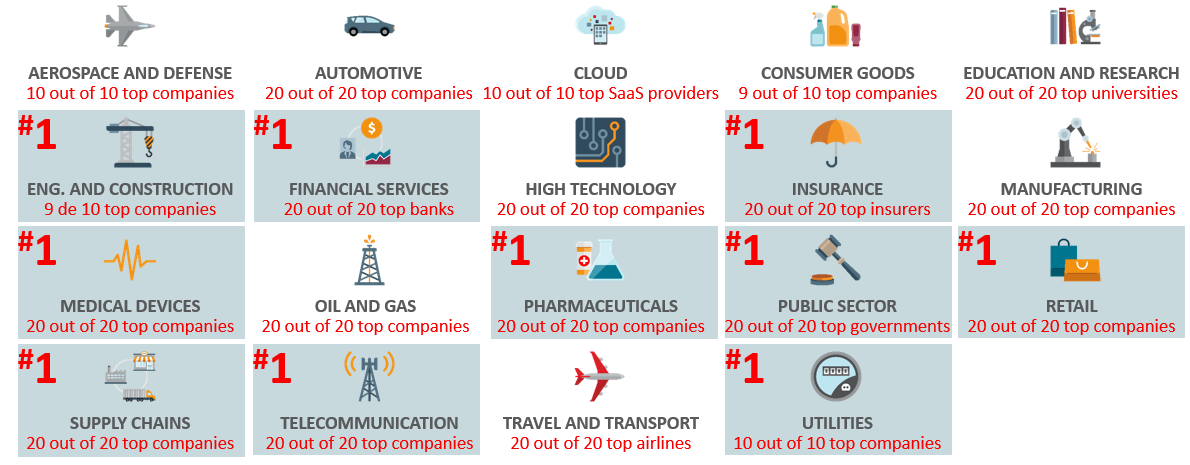
\includegraphics[width=0.8\textwidth]{chapitre1/Figures/OracleCustumers.PNG}
  \caption{Les clients d'Oracle}
\end{figure}

\subsection{Présentation de ORACLE LABS}
Oracle Labs (anciennement Sun Microsystems Laboratoires, ou Sun Labs) est une branche de recherche et développement d'Oracle Corporation. Oracle Labs a été créés lorsque Oracle a acquis Sun Microsystems [b.6].\\
\begin{figure}[H]  
  \centering
    
\includegraphics[width=0.5\textwidth]{chapitre1/Figures/OracleLabs.png}
\end{figure}
Oracle Labs et la source de plusieurs projets qui ont impacté la technologie d’aujourd’hui comme Java, Oracle Labs travaille aussi sur d’autres projets qui ont un grand potentiel de devenir l'état de l'art en quelques années, le plus connus est GraalVM [b.7].\\

GraalVM explore des nouvelles architectures pour les machines virtuelles (VM). La vision de GraalVM est de créer une seule VM qui offre des performances élevées pour tous les langages de programmation, facilitant ainsi la communication entre les programmes. Cette architecture supporte un outil unifié d'analyse des langages pour une meilleure maintenabilité et son intégration rendrait la VM omniprésente dans la pile de développement.\\

Cette nouvelle architecture des machines virtuelles est déjà utilisée par des grand sociétés tel que AliBaba vu son potentiel.\\

\begin{figure}[H]  
  \centering
    
\includegraphics[width=0.5\textwidth]{chapitre1/Figures/GraalVM.png}
  \caption{Logo GraalVM}
\end{figure}

Le second plus important projet sur lequel Oracle Labs travaille et PGX le projet dont j’étais membre dans mon stage PFE. PGX est une boîte à outils pour l'analyse des graphes qui permet à la fois d'exécuter des algorithmes tels que le PageRank sur les graphes, et d'effectuer des requêtes semblables à SQL mais sur les graphes, on détaillera dans la suite de ce rapport l’Outil PGX.
\section{Contexte du projet}

\subsection{Présentation du projet et ces objectives}

\begin{figure}[h!]  
  \centering
    
\includegraphics[width=0.7\textwidth]{chapitre1/Figures/PGX-logo.png}
\end{figure}

Les bases de données de graphes, est parmi les derniers outils nés pour les data scientistes, et data analystes après le BigData il y a quelques années. Ils ont vu le jour pour résoudre des problèmes d’extraction et de traitement des données précédemment difficiles à approcher avec les outils déjà existants. Vous pouvez certainement faire le même type d'analyse qu'une base de données de graphes vous permet de faire sur votre base de données relationnelle. Mais vous devrez écrire des tonnes de code et il sera probablement assez mal exécuté.\\
Selon le classement [16] Gartner en 2019, les outils de traitements et analyse des graphes constitue la tendance numéro 5 dans le domaine d’analyse des données et explique : \\
« L'application du traitement des graphes et des SGBD de graphes connaîtra une croissance annuelle de 100\% jusqu'en 2022 afin d'accélérer continuellement la préparation des données et de permettre une science des données plus complexe et plus adaptative. \\
Les entrepôts de données des graphes peuvent efficacement modéliser, explorer et interroger des données avec des interrelations complexes. Mais le besoin de compétences spécialisées a limité leur adoption jusqu'à présent.\\
L'analyse des graphes se développera dans les prochaines années en raison de la nécessité de poser des questions complexes à travers des données complexes, ce qui n'est pas toujours pratique ou même possible à l'échelle en utilisant des requêtes SQL »\\
Oracle a rejoint ce mouvement avec sa solution de graphes de propriétés : PGX, l'acronyme de Parallel Graph AnalytiX. PGX lui-même se manifeste sous deux formes, PGX.SM (PGX Shared Memory) et PGX.D (PGX Distributed), à chacun ces avantages. Cette flexibilité permet à Oracle d’être un grand compétiteur.\\
GX peut être un outil d’analyse des graphes autonome, et il est aussi le cerveau des implémentations de graphe qu'Oracle utilise dans divers outils comme FCC Studio, Data studio et autres. Cet outil qui effectue des opérations sur les graphes en mémoire, mais ne fournit pas de stockage direct (Figure 2). Le stockage (lecture et écriture) est fourni par des solutions externes comme les fichiers du système (filesystem), SQL (database), NoSQL, Spark et HDFS.\\

\begin{figure}[h!]  
  \centering
    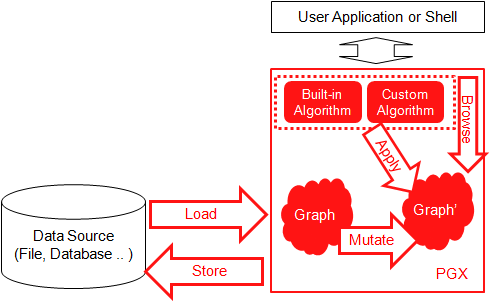
\includegraphics[width=0.7\textwidth]{chapitre1/Figures/pgx_overview.png}
  \caption{Architecture PGX}
\end{figure}

\subsection{Compétiteurs de PGX}

Orcale n’est pas l’unique utile de traitement des graphes sur le marché, Il y a plusieurs compétiteurs industriels ainsi que ceux académique. Dans la suite de cette section je vais montrer quelques comparaisons entre PGX et d’autres systémies.\\
\begin{itemize}
\item PGX offre plus des facilités pour les analystes pour augmenter la productivité comme montre le tableau suivant :
\begin{table}[h!]  
  \centering
    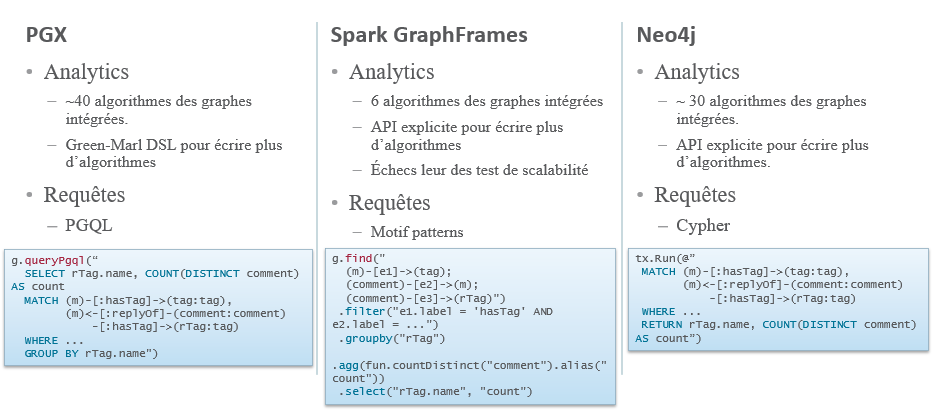
\includegraphics[width=1.15\textwidth]{chapitre1/Figures/FonctionalitesPGX.png}
  \caption{Comparaison des fonctionnalités entre PGX, GraphFrames et Neo4j [15]}
\end{table}

\item PGX offre une meilleure performance par rapport aux autres systèmes.

\begin{table}[h!]  
  \centering
    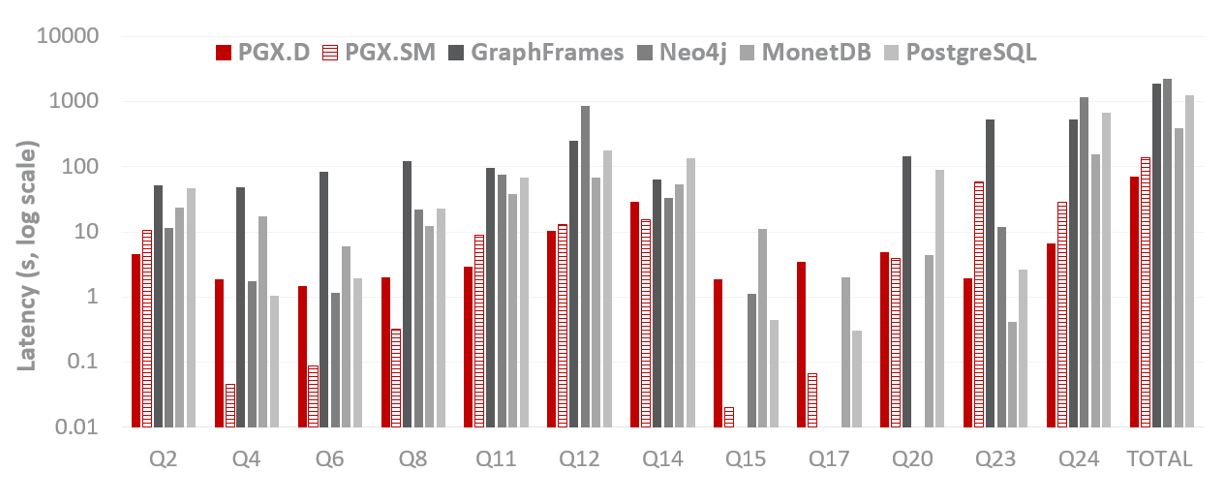
\includegraphics[width=1.15\textwidth]{chapitre1/Figures/BenchmarkLDBC.png}
  \caption{Benchmark LDBC; 8 machines pour PGX.D et GraphFrames}
\end{table}
\end{itemize}

\subsection{Conduite du projet}
La conduite de projet était cadrée par l’approche agile SCRUM, elle est l’une des méthodologies les plus utilisées dans le développement logiciel. SCRUM étant une approche qui suit la méthodologie agile, implique la participation active du client tout au long du projet.\\
L’approche SCRUM et choisie vue ces avantages, à citer la diminution de la possibilité de livrer un projet complet qui ne répond pas ou besoins du client, puisque celui-ci ca toujours une vision imprécise qui s’améliore au cours du temps.\\
SCRUM répondre au besoin et aux exigences du client en termes de qualité et de fonctionnement, par ça flexibilité et adaptabilité aux évolutions éventuelles des besoins métiers. La démarche à choisir devrait également assurer l’implication du client dans le projet, et ceci en livrant à la fin de chaque itération un produit fonctionnel et testable.\\
Le feedback devra être pris en considération dans les versions suivantes de l’itération.\\

\begin{figure}[h!]  
  \centering
    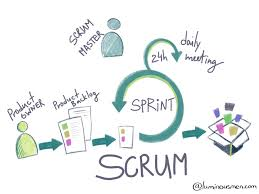
\includegraphics[width=0.7\textwidth]{chapitre1/Figures/SCRUM.jpg}
  \caption{Processus SCRUM}
\end{figure}

Pour bien suivre le projet et implémenter la méthode SCRUM de manière efficace, L’équipe PGX opte pour les solutions ATLASSIAN suivantes :
\begin{itemize}
\item Confluence : Pour documenter, discuter et partager tout information lié ou projet comme la conception, et l’analyse des nouvelles fonctionnalités. 
\item JIRA : Pour affecter des tâches à chaque membre de l’équipe, suivre le backlog, et l’état du sprint.
\item BitBucket : Une alternative a github et gitlab, qui implémente le protocole GIT la collaboration efficace des équipes des tous les tailles.
\end{itemize}
Ces trois solutions sont interdépendantes et permettent d’automatiser certaines tâches, comme la modification de l’état du ticket en JIRA selon l’état de celle-ci dans BitBucket.\\

\subsection{Diagramme de Gante}
\begin{figure}[h!]  
  \centering
    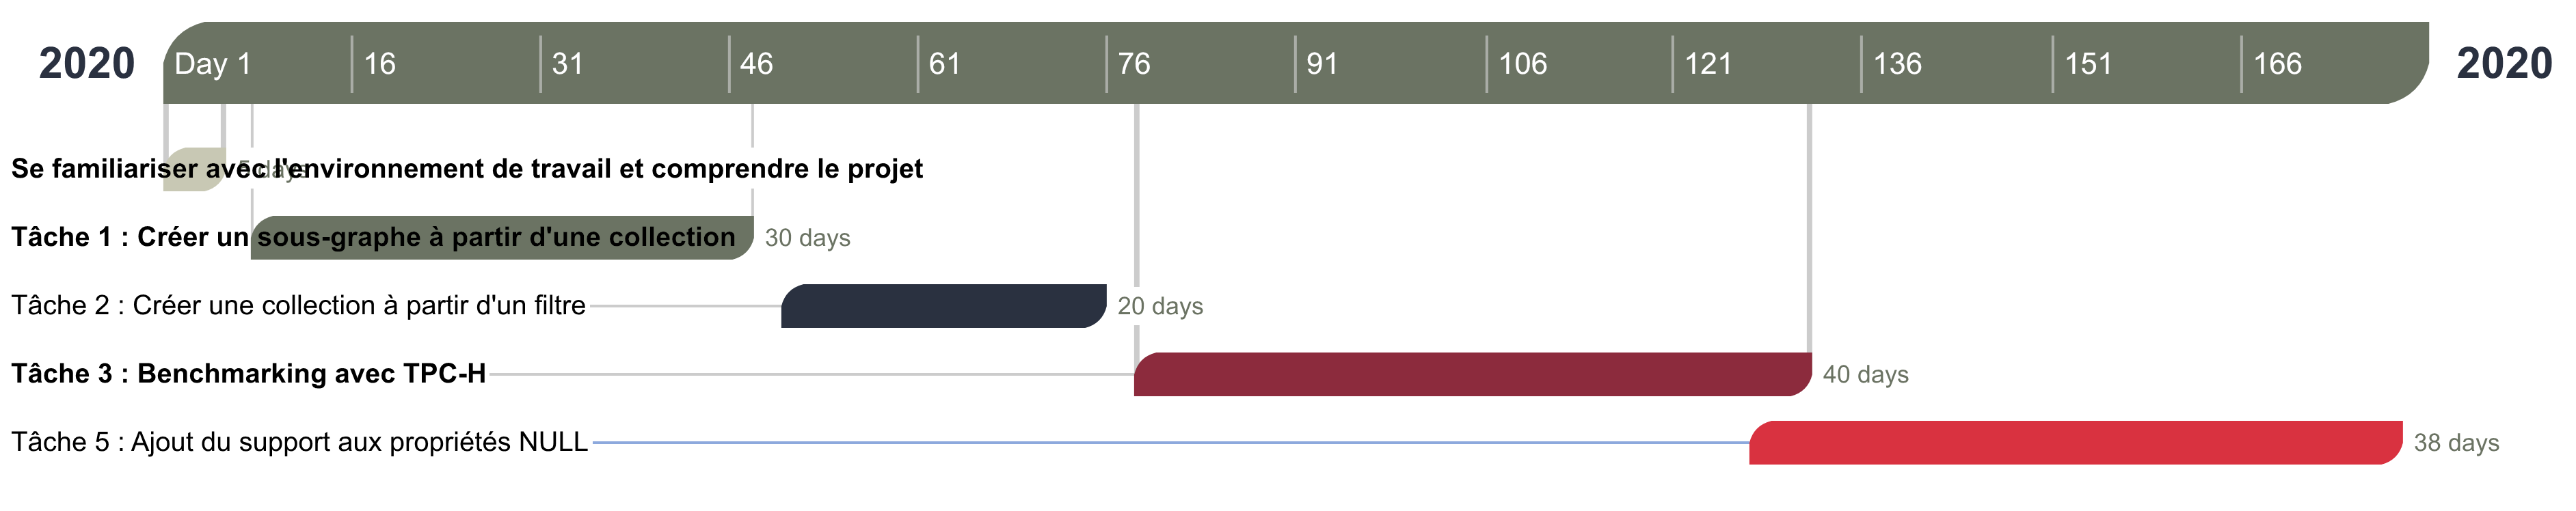
\includegraphics[width=1.2\textwidth]{chapitre1/Figures/PlanningRoadmap.png}
  \caption{Diagramme de Gante de déroulement du stage}
\end{figure}
\chapter{Traitement des graphes distribuées}
Le traitement des graphes distribuées qui constitue l’axe principale du projet PGX, est un sujet récent, qui n’a vu le jour que dans les deux dernières décennies. Cet intérêt par ce nouveau domaine et dû principalement à l’explosion des utilisateurs d’internet en générale et des réseaux sociaux en particulier. Ce sujet est assez complexe et avancé, c’est pour cette raison qu’il faut définir quelques notions que l’englobe avant d’aller plus loin.\\

\section{Qu’est-ce qu’un graph}
Un graphe est un modèle abstrait de dessins de réseaux reliant des objets [b.8]. Ces modèles sont constitués par la donnée de sommets (aussi appelés nœuds), et d'arêtes (aussi appelées liens ou relation) entre ces sommets ; ces arêtes sont parfois non-symétriques (les graphes sont alors dits orientés) et sont appelés des flèches.\\

\begin{figure}[H]  
  \centering
    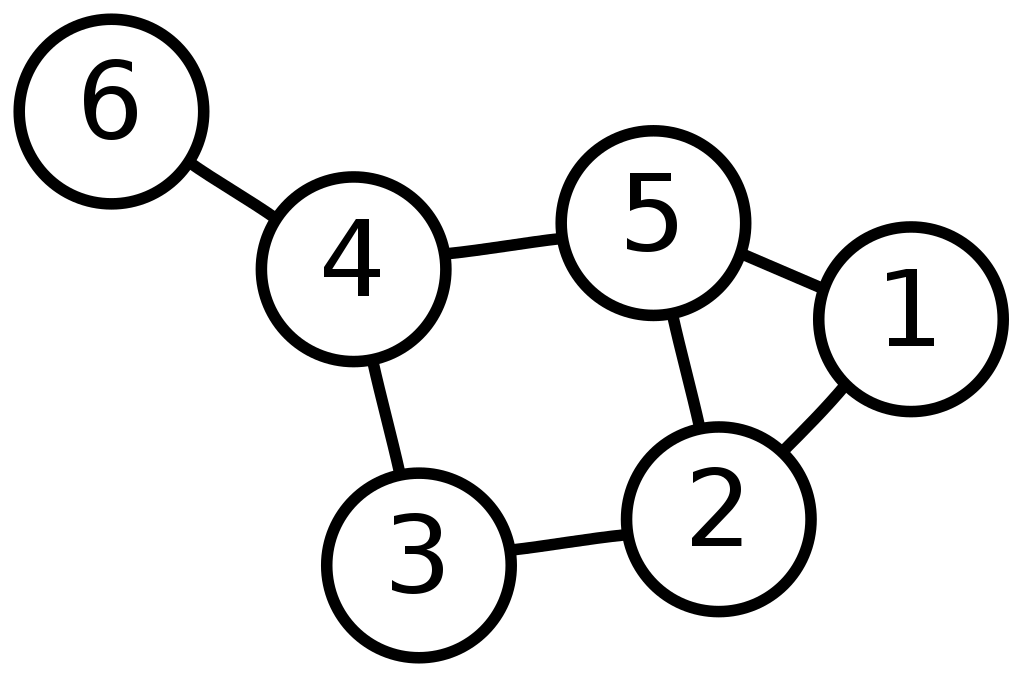
\includegraphics[width=0.5 \textwidth]{chapitre2/Figures/GraphNonOriontee.png}
  \caption{Graphe non orientée}
  \centering
    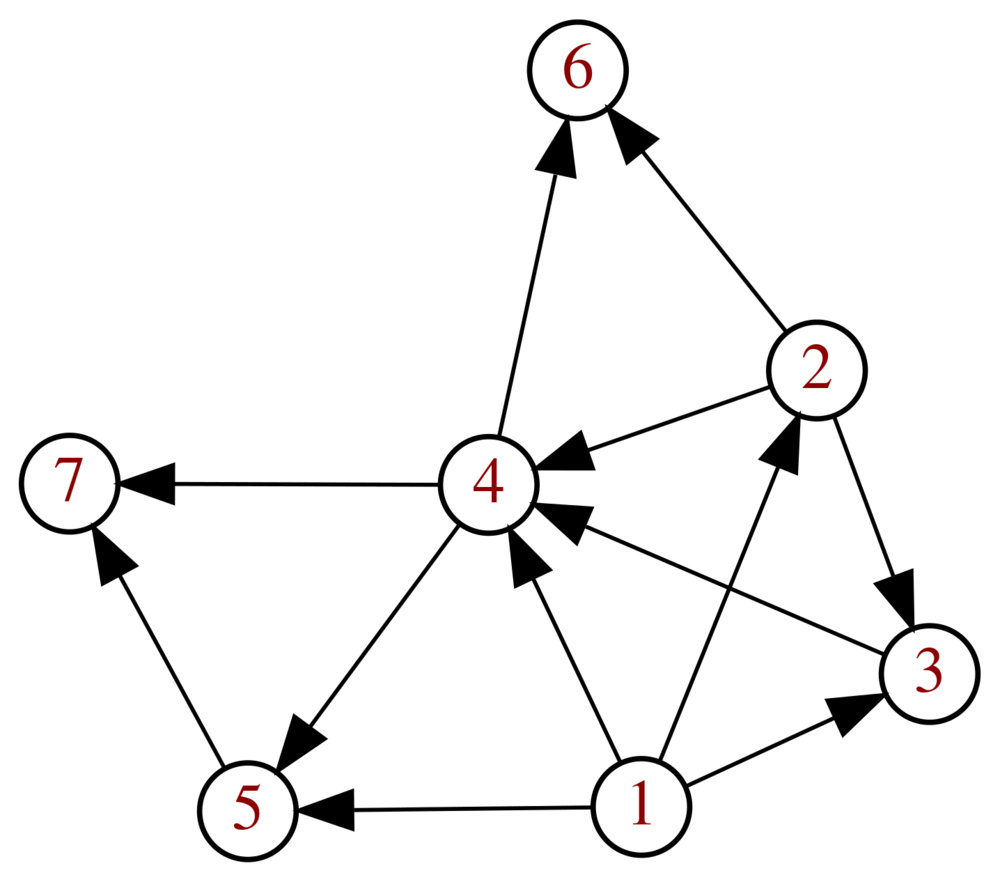
\includegraphics[width=0.5 \textwidth]{chapitre2/Figures/GraphOriontee.png}
  \caption{Graphe orientée}
\end{figure}

On ne peut pas parler des graphes dans le contexte académique sans parler de la théorie des graphes, c’est la discipline mathématique et informatique qui étudie les graphes. La théorie des graphes il a comme origine le mathématicien suisse Leonhard Euler, qui en 1735 a présenté à l'Académie de Saint-Pétersbourg un article qui traitait le problème des sept ponts de Königsberg. Le problème consistait à traverser une ville appelée Königsberg, cette ville est construite autour de deux îles situées sur un fleuve et reliées entre elles par un pont. Six autres ponts relient les rives de la rivière à l'une ou l'autre des deux îles, comme représentés dans la figure ci dessus. Le problème consiste à déterminer s'il existe ou non une promenade dans les rues de Königsberg permettant, à partir d'un point de départ au choix, de passer une et une seule fois par chaque pont, et de revenir à son point de départ, étant entendu qu'on ne peut traverser la rivière qu'en passant sur les ponts.\\

\begin{figure}[H]  
  \centering
    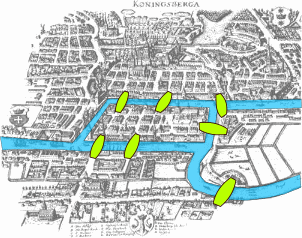
\includegraphics[width=0.4 \textwidth]{chapitre2/Figures/Konigsberg_bridges.png}
  \caption{Ville de Königsberg et ces sept ponts}
  \centering
    \includegraphics[width=0.4 \textwidth]{chapitre2/Figures/Königsberg_graph.svg.png}
  \caption{Modéle en graphe orionté de la ville de Königsberg}
\end{figure}

Les algorithmes élaborés pour résoudre des problèmes concernant les objets de cette théorie ont de nombreuses applications dans tous les domaines liés à la notion de réseau (réseau social, réseau informatique, télécommunications, etc.) et dans bien d'autres domaines.
\input{chapitre2/definitionProperyGraph}
\section{Qu’est-ce qu’un graph distribué}
Pour comprendre ce qu’un graph distribué, il faut d’abord qu’est-ce que un système distribuée, par-ce-que un graphe distribuée n’est que un cas particulier des systèmes distribuées.\\
Un système distribué [14], également connu sous le nom de "calcul distribué", est un système comportant de multiples composants situés sur différentes machines qui communiquent et coordonnent des actions afin d'apparaître comme un seul système cohérent pour l'utilisateur final.\\
Un système distribué, au contraire d’un système centralisé, son état a un moment t est stocké dans plusieurs machines, c’est-à-dire que pour savoir l’état du système à un certain moment il faut savoir l’état des tous les machines que le compose. Ces caractéristiques introduisissent plusieurs avantages ainsi que des inconvénients :\\

\textbf{Les avantages :}
\begin{itemize}[label=\textbullet]
\item  Scalabilité horizontale : Comme le calcul se fait indépendamment sur chaque nœud, il est facile et généralement peu coûteux d'ajouter des nœuds et des fonctionnalités supplémentaires si nécessaire.\\
\item  Fiabilité : la plupart des systèmes distribués sont tolérants aux pannes car ils peuvent être constitués de centaines de nœuds qui fonctionnent ensemble. Le système ne subit généralement pas de perturbations si un nombre de machines tombe en panne généralement le système distribué qu’utilise des algorithmes de consensus robustes tel que RAFT [13] ou PAXOS, peuvent se permettre jusqu’à N / 2 machines en panne si le nombre des machines est N + 1.
\item  Performance : Les systèmes distribués sont extrêmement efficaces car les charges de travail peuvent être fragmentées et envoyées à plusieurs machines. Sauf que la tâche difficile dans la plupart des systèmes consiste à comment le fragmenter, de manière à ce que l’avantage obtenu dépasse les désavantages, ceci reste encore un sujet de recherche intense.
\end{itemize}

\textbf{Les désavantages :}
\begin{itemize}[label=\textbullet]
\item  Ordonnancement : Un système distribué doit décider quelles tâches doivent être exécutées, quand et où elles doivent être exécutées. Les ordonnanceurs ont finalement des limites, ce qui entraîne une sous-utilisation du matériel et des durées d'exécution imprévisibles.
\item  Latence : Plus votre système est largement distribué, plus vous pouvez connaître une latence dans les communications. Cela conduit souvent les équipes à faire des compromis entre disponibilité, cohérence et latence.
\item  Observabilité : La collecte, le traitement, la présentation et le suivi des mesures d'utilisation du matériel pour les grands clusters constituent un défi important.
\end{itemize}

Dans le même contexte les systèmes distribuées peuvent se manifester sous forme de plusieurs architectures voici deux :\\
\begin{itemize}[label=\textbullet]
\item  Peer-to-peer : Il n'y a pas de machines supplémentaires utilisées pour fournir des services ou gérer des ressources. Les responsabilités sont uniformément réparties entre les machines du système, appelées "pairs", qui peuvent servir soit de client, soit de serveur. BitTorrent est l’un des exemples les plus connues car chaque machine que l’installe devient fournisseur de service pour les autres utilisateurs.
\item  Les clusters : sont des systèmes distribués fabriqués à partir de composants de commodité (ordinateur personnel, serveur, Raspberry PI …etc.). Les nœuds sont des machines contenant un ou quelques processeurs, de la mémoire RAM et souvent du stockage sur disque.
Les nœuds sont reliés par une interconnexion de produits, qui est disponible en plusieurs formes, notamment Gigabit Ethernet et Infiniband. En utilisant de composants de commodité, les clusters ont un rapport prix/performance exceptionnel par rapport à la plupart des autres formes d'informatique haut de gamme.
PGX Distribuée en mode développement tire profit de cette architecture, car elle offre la meilleure performance due à la petite latence qui génère parce que les machines sont interconnectées directement.
\item  ...
\end{itemize}

Maintenant qu’on a compris ce que un système distribuée, et que un graph distribuée et l’un des systèmes il faut décrire les spécificités de ce type des graphes, ces avantages et ces inconvénients.

\begin{figure}[h!]  
  \centering
    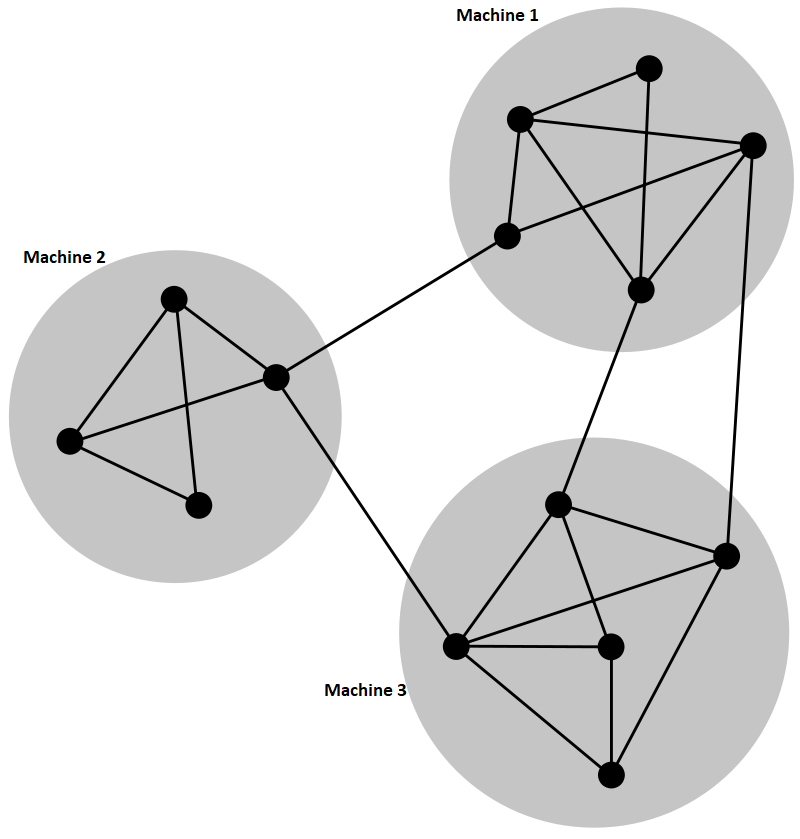
\includegraphics[width=1\textwidth]{chapitre2/Figures/Network_Community_Structure.svg.png}
  \caption{Exemple d'un graphe distribué sur trois machines}
\end{figure}

Si on observe bien on peut remarquer que les graphes sont partout dans notre entourage, le plus simple exemple sont les routes qui interconnecte les villes, les villes seront modélisées en sommets et les routes comme les arêtes et à partir de cette modélisation en peut extraire un grand nombre d’informations grâce aux outils développes par la théorie des graphes. L’algorithme de Dijkstra étant un exemple d’algorithme que donc le cas idéal (Le graphe est statique, pas d’embouteillages, vitesse fixe …etc.), permet d’extraire le chemin le plus court entre deux villes en un temps polynomial. Dans le cas ou le graphe et petite en peut implémenter, ce algorithme pour s’exécuter sur une seule machine et on auras le résultat prévue, mais lorsque le graphe ne peut pas être chargé sur une seule machine il faut opter pour un graphe distribuée.\\
Implémenter un graphe distribué n’est pas une tâche simple, la plus grande problématique consiste à le partitionner en des sous-graphes faiblement couplé pour diminuer ainsi la communication entre les machines qui est souvent la source de plus grande perte de performance. Il existe plusieurs méthodes et techniques pour partitionner un graphe, tous ce concentre sur le fait de démineur les connexion entre les sous-graphes dans chaque machine et en même temps d’assurer que la charge est balancé c’est-à dire que la différence entre le nombre des sommets et arrêts dans chaque nœud est petite.\\
Parmi les techniques les plus utilisée en trouve DFS ou BFS pour trouver toutes les composantes faiblement et fortement connectées, et l’utilisation des sommets fantôme (Ghost nodes/vertices) pour le sommet qui sont partagées entre les machines. Ces calcules préalables ainsi génère des coûts indirects, ce qui rend le chargement du graphe en sa forme final qui peut être exploité par l’utilisateur plus lente, en verra dans le chapitre du benchmarking avec TPC-H, comment j’ai souffert avec ce problème et comment j’ai pu réduire ce temps significativement spécifiquement pour la tâche que j’avais en main.\\

\section{Le traitement des graphes distribuées}
L'analyse des graphes est un ensemble de techniques analytiques qui permettent d'explorer les relations entre des entités qui nous intéressent, telles que des organisations, des personnes et des transactions [12]. Les entrepôts de données de graphes peuvent efficacement modéliser, explorer et extraire des données avec des interrelations complexes. L'analyse des graphes et prometteuse, en raison de la nécessité de poser des questions complexes à travers des données complexes, ce qui n'est pas toujours pratique ni même possible à l'échelle en utilisant des requêtes SQL.\\
Il y a trois méthodes principales pour approcher le traitement des graphes :

\begin{itemize}[label=\textbullet]
\item  Computational graph analytics : Itérer le graphe plusieurs fois et calculer certaines propriétés mathématiques. L’exemple le plus connue pour utiliser cette approche et l’algorithme PageRank de Google, qui permet d’ordonner les pages web selon priorité. PageRank modélise le web comme un graphe ou les pages sont les sommets et les liens URL entre les pages sont les arrêts.
\item  Graph querying and pattern matching : Exécuter des requetés sur le graphe pour trouver des sous-graphes qui correspondent au pattern spécifié par l’utilisateur. Cette approche est similaire aux requêtes SQL sur base des données relationnels.
\item  Graph ML : Il consiste à utiliser les algorithmes du machine learning pour trouver des informations structurelles latente dans les graphes, comme les clusters des personnes avec des intérêts similaires dans un graph sociale.
\end{itemize}

PGX support premièrement les deux premières approches, la première puisque il offre plus que 40 algorithmes implémentés et laisse la possibilité aux utilisateurs aussi d’implémenter leur propre algorithmes via le Domain Spécific Language(DSL) GreenMarl.

\chapter{Filtrage des graphes}
\section{Introduction}
Le filtrage des graphes est l'une des caractéristiques essentielles que tout système d'analyse des graphes devrait pouvoir fournir, car il ouvre les portes à de nombreuses applications, pour n'en citer que quelques-unes, un analyste de données pourrait vouloir éliminer toutes les valeurs extrêmes qui peuvent influencer l'exactitude de ses résultats.\\
Mon but pendant le stage était d'ajouter des capacités de filtrage supplémentaires, alors que la plupart des infrastructures étaient déjà fournies pour moi, en particulier ce que je devais faire est d'utiliser ces infrastructures de la bonne manière pour atteindre mon objectif.\\
PGX.D prenait déjà en charge les filtres basés sur des expressions de filtrage, mais il manquait de nombreuses autres possibilités capabilités, comme le filtrage basé sur une collection ou un result-set.\\
Dans la suite de ce chapitre, je me concentrerai sur deux types de filtres que j'ai mis en œuvre, le premier consiste à créer un sous-graphe basé sur une collection, et le second consiste en l'opération inverse, c'est-à-dire créer une collection basée sur un filtre de sous-graphe, et à la fin, je présenterai certains des efforts que j'ai faits pour mettre en œuvre le filtrage basé sur un result-set.\\

\section{Conception du filtrage des graphes en mode distribué (général).}
Le flux d'évaluation d'un filtre en PGX.D peut se modéliser comme suit :
\begin{figure}[H]  
  \centering
    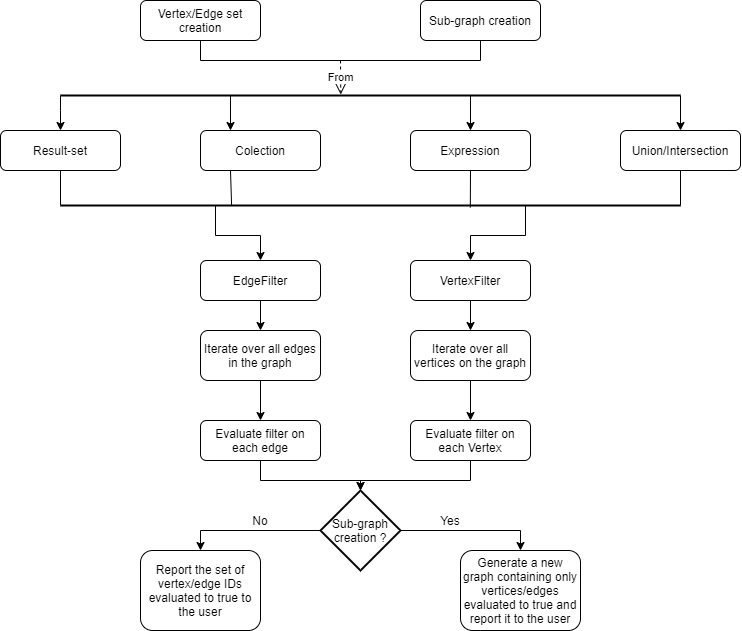
\includegraphics[width=1\textwidth]{chapitre3/Figures/Set-SubGraph-creation.png}
  \caption{Diagramme de flux de l'opération du filtrage}
\end{figure}

La création d'une collection de sommets/arêtes dans PGX peut se faire par plusieurs types de filtres :

\begin{itemize}[label=\textbullet]
\item  À partir d'un result-set : le résultat de l'exécution d'une requête PGQL.
\item  Une collection : Elle peut être générée manuellement ou à partir d'un filtre de sous-graphes (ce dont nous parlerons plus tard)
\item  Une expression : C'est une requête spéciale, qui est traduite en requête PGQL et ensuite exécutée.
\item  Une Union/Intersection : C'est le cas lorsque vous voulez appliquer plusieurs filtres à la fois.
\end{itemize}

Chacun de ces filtres peut être spécifié soit pour les arêtes, soit pour les sommets, et dans ce cas, il sera appelé VertexFilter ou EdgeFilter en fonction de la cible que nous spécifions dans notre requête.\\

\section{Le filtre est un VertexFilter(Filtre des sommets)}
Pour povoir filtrer un graphe par ces sommets, deux étapes essentielles sont nécessaires dans PGX:

\begin{enumerate}[label=\arabic*)]
\item  Pour chaque sommet du graphe, évaluez le filtre, placez un indicateur temporaire sur ce sommet, cette indicateur est un booléen qui précise si le sommet doit être conservé dans le sous-graph résultant, et nous envoyons le résultat de l'évaluation à tous les sommets entrants, ce qui réduit la quantité de messages à envoyer ("dans le cas où deux sommets ne se trouvent pas dans la même machine”):
\begin{figure}[H]  
  \centering
    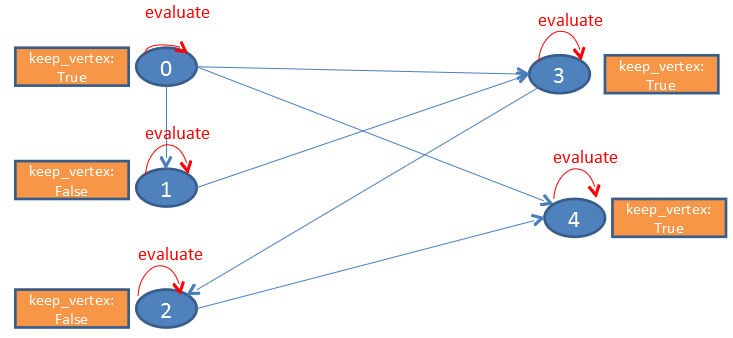
\includegraphics[width=1\textwidth]{chapitre3/Figures/VertexFilter1.png}
  \caption{1re étape de l'évaluation d'un filtre des sommets}
\end{figure}

\item  Chaque sommet ayant un bord sortant vers un autre sommet qui a été évalué comme vrai recevra un message de ce sommet pour potentiellement garder l'arête qui leur relié dans le cas où il serait évalué comme vrai.
\begin{figure}[H]  
  \centering
    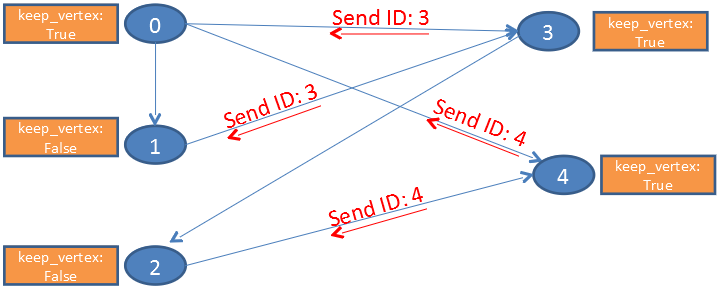
\includegraphics[width=1\textwidth]{chapitre3/Figures/VertexFilter2.png}
  \caption{2éme étape de l'évaluation d'un filtre des sommets}
\end{figure}
\end{enumerate}

\section{Le filtre est un EdgeFilter(Filtre des arêtes)}
Une arête est la composition de deux sommets (source, destination). Nous avons donc besoin d'informations sur les deux sommets pour pouvoir évaluer le filtre, ce qui implique plus d'étapes. Aussi il faut noter que l'évaluation du filtre ne se fait que sur la source de l'arête et non sur la destination :\\
\textbf{On à quatre étapes :}
\begin{enumerate}[label=\arabic*)]
\item  Envoyer les propriétés nécessaires à l'évaluation du filtre d'arête à la source (donc, à tous les voisins entrants de la destination), puisque les propriétés sont stockées dans les machines possédant le sommet
\begin{figure}[H]  
  \centering
    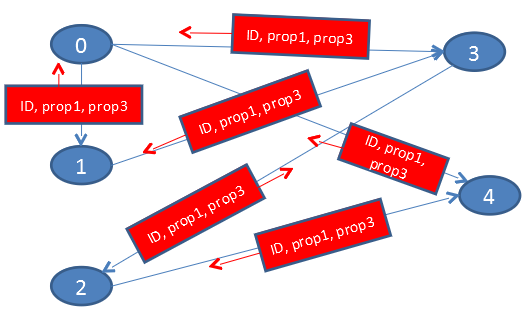
\includegraphics[width=0.8\textwidth]{chapitre3/Figures/EdgeFilter1.png}
  \caption{1er étape de l'évaluation d'un filtre des arêtes}
\end{figure}

\item  Pour chaque entrée de données de filtrage (propriétés, et ID de destination) arrivant des sommets de destination des arêtes sortantes du sommet source actuel :
    \begin{enumerate}[label=\alph*)]
    \item  Nous déterminons l'arête correspondante pointant vers la destination.
    \item  Nous évaluons le filtre à l'aide des données que nous avons reçues.
    \item  Si le filtre est évalué positivement, nous fixons un indicateur temporaire à la valeur "true" dans la source et l'arête évaluée.
    \item  Pour tous les sommets de destination, si le filtre est évalué positivement, envoyez un message qui indique que nous voulons le garder.
    \end{enumerate}
\begin{figure}[H]  
  \centering
    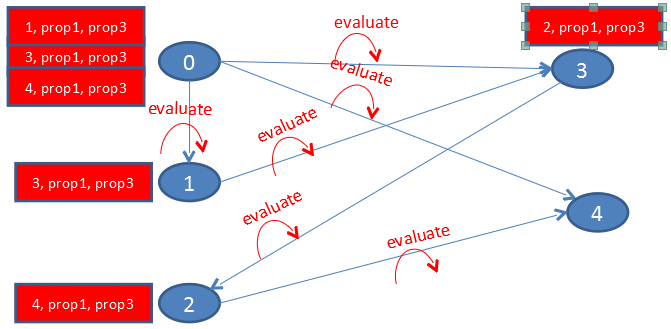
\includegraphics[width=1\textwidth]{chapitre3/Figures/EdgeFilter2.png}
  \caption{2éme étape de l'évaluation d'un filtre des sommets}
\end{figure}

\item  Lorsque le sommet de destination reçoit un message "keep", un indicateur est fixé à true pour garder le sommet.
\begin{figure}[H]
  \centering
    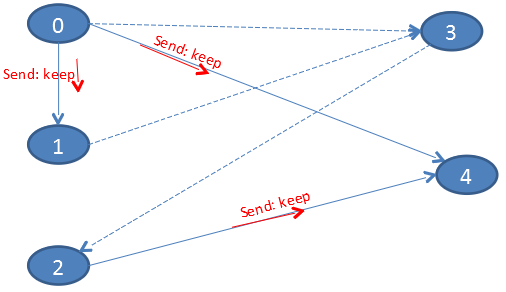
\includegraphics[width=1\textwidth]{chapitre3/Figures/EdgeFilter3.png}
  \caption{3éme étape de l'évaluation d'un filtre des arêtes}
\end{figure}

\item  Dernière étape (Étape commune entre le deux types de filtres EdgeFilter et VertexFilter ):
Nous parcourons tous les sommets/arêtes du graphe et si l'indicateur temporaire de à comme valeur "true", nous les ajoutons à un nouveau sous-graphe. Et enfin, nous communiquons le sous-graphe au client.
\end{enumerate}

\section{Conception de l'évaluation du filtrage (Filtre basé sur une collection)}
\subsection{Aperçu}
Une collection est un ensemble d'éléments homogènes, dans notre contexte, ces éléments sont les ID des sommets que nous voulons conserver dans le sous-graph résultant.\\
La création d'une collection peut se faire de plusieurs façons dans PGX (manuellement en utilisant l'API de la collection, en utilisant un algorithme ...etc.) pour présenter notre solution, nous utiliserons une collection construite manuellement pour filtrer un simple graphe.\\
À partir de cette collection, nous créons un filtre de sommet ou d'arête que nous appliquons sur le graphe original. En mode distribué, cela implique que la collection sera également distribuée, dans notre système, nous nous assurons que l'ID de chaque sommet, s'il est correct, est placé dans la sous-collection qui résidera dans la machine contenant ce sommet.\\

\begin{figure}[H]  
  \centering
    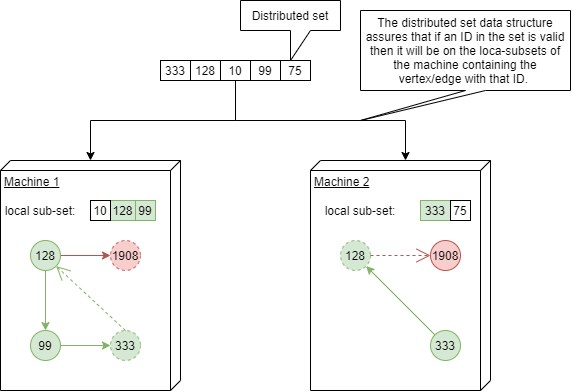
\includegraphics[width=1\textwidth]{chapitre3/Figures/SubgraphFromCollection.png}
  \caption{Exemple qui démontre l'exécution d'un filtre basé sur une collection}
\end{figure}

\subsection{Implémentation}
\begin{enumerate}[label=\arabic*)]
\item  On itère sur le graphe, sommet par sommet ou arête par arête selon le type de filtre.
\item  Nous vérifions si l'ID du sommet actuel est présent dans la collection locale ou non, s'il existe, le filtre l'évalue comme vrai et nous fixons l'indicateur pour garder le sommet ou l'arête comme nous l'avons décrit précédemment.
\end{enumerate}
Cela est fait de manière concurrente, mais comme nous ne faisons que lire, nous n'avons pas eu de problèmes de synchronisation.


\section{Conception de l'évaluation du filtrage (Création d’une collection à partir d’un filtre de sous graphe)}
Nous évaluons le filtre sur le graphe sans la dernière étape, en créant le nouveau sous-graph. Au lieu de cela, chaque fois qu'un sommet ou une arête est évalué comme vrai, nous l'ajoutons à une collection distribuée.\\
\begin{figure}[H]  
  \centering
    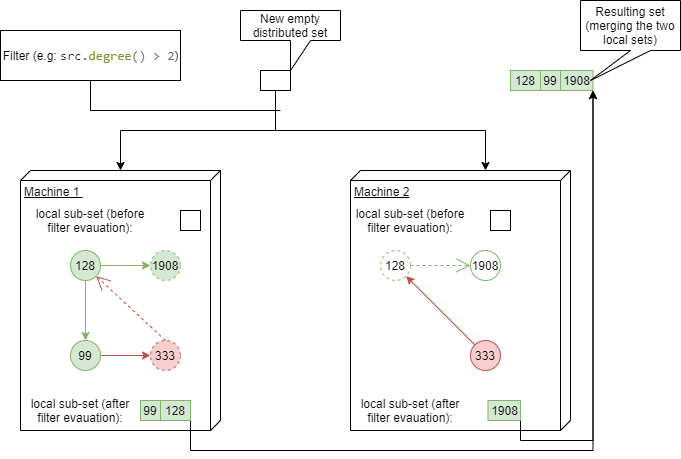
\includegraphics[width=1\textwidth]{chapitre3/Figures/CreateSetFromFilter.png}
  \caption{Exemple qui démontre l'extraction d'une collection à partir d'un autre filtre (basé sur une expression dans ce cas)}
\end{figure}
\chapter{Support des propriétés NULL dans les frames en PGX.}
\section{Introduction}
NULL est l'un des sujets délicats que les programmeurs doivent traiter. Les objets ou valeurs NULL peuvent apparaître partout dans le code, mais la raison principale est d'avoir des valeurs optionnelles, par exemple dans une base de données SQL. Si nous voulons éviter les valeurs NULL, nous devons alors remplir chaque table avec tous les champs existants et fixer les champs ajoutés à une valeur par défaut, ce qui présente de nombreux inconvénients comme l'augmentation de la consommation de mémoire, la difficulté de choisir ces valeurs par défaut, et peut également générer des bugs et des résultats incorrects si ces valeurs magiques par défaut s'avèrent réelles. De nombreuses questions se posent alors, comme par exemple si une valeur est optionnelle et n'est pas fixée par l'utilisateur, que faut-il y mettre à la place ? Comment procéder si l'exécution rencontre un pointeur nul ? Quel est le résultat d'une opération contenant des valeurs NULL ?
\section{Problème en PGX.D}
PGX.D ne prend pas en charge les valeurs NULL, contrairement à PGX.SM, mais comme nous ne prenons actuellement en charge que les graphes homogènes, cela signifie que tous les sommets/arêtes auront les mêmes propriétés.  C'est pourquoi nous avons utilisé une solution de contournement, qui consiste à avoir des valeurs par défaut au cas où le sommet ou l'arête n'est pas censé avoir cette propriété, ces valeurs par défaut sont choisies avec soin pour conserver l'exactitude des opérations qui les utilisent. Cependant, afin de permettre le support des graphes hétérogènes, où les sommets/arêtes n'ont pas tous les types de propriétés, il sera davantage nécessaire de supporter les valeurs nulles.\\
Par exemple, une requête PGQL sur des graphes homogènes (pas de support des propriétés NULL, mais des valeurs par défaut sont utilisées) donne le résultat suivant:

\begin{figure}[H]  
  \centering
    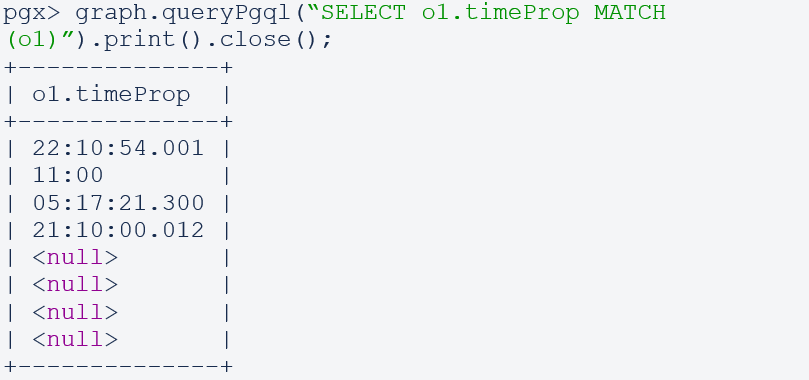
\includegraphics[width=1\textwidth]{chapitre4/Figures/PGXD_query.png}
\end{figure}

En revanche, dans les graphes hétérogènes, avec le support NULL, les valeurs par défaut sont remplacées par "<null>":

\begin{figure}[H]  
  \centering
    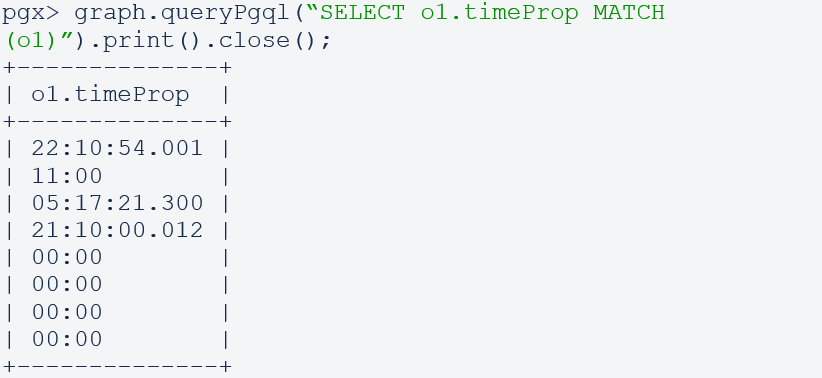
\includegraphics[width=1\textwidth]{chapitre4/Figures/PGX_query.png}
\end{figure}

L'implémentation de NULL n'est pas simple et dépend de beaucoup de facteurs, principalement du langage que vous utilisez et du système que vous implémentez puisque ce dernier peut se soucier ou non de la mémoire et/ou des performances en matière de temps. Dans notre cas, le temps et le rendement de la mémoire sont essentiels, car la charge de travail est énorme et la taille d’un frame peut atteindre des milliards, voire des trillions de lignes.\\

\section{Solution}
Comme nous l'avons déjà dit, les principales préoccupations qui ont motivé nos choix de conception ont été les performances en matière de temps et de mémoire. C'est pourquoi, étant donné la manière dont notre système a été mis en œuvre, nous avons décidé que pour chaque élément, nous ajoutons un indicateur, qui permet de savoir si un élément est NUL ou non. La question qui se pose alors est de savoir quelle structure de données ou quel type de données nous devons utiliser, tel que la modification de ces données, se fera avec un minimum de temps et leur stockage sera aussi minimal que possible.\\
Comme le système est implémenté en C++, l'un des outils les plus faciles à mettre en œuvre et à utiliser est la classe de tableau de bits (std ::bitset)[b.1] de la Standard Template Library (STL), car elle présente les avantages suivants:

\textbf{Avantages :}
\begin{itemize}[label=\textbullet]
\item  Permet une allocation par bits et un accès aléatoire comme un tableau.
\item  Plusieurs méthodes prédéfinies pour le manipuler, comme set(), reset() et flip().
\item  Peut être entièrement mis en cache dans un cache L1 si la taille n'est pas énorme.
\end{itemize}

\textbf{Inconvénients :}
\begin{itemize}[label=\textbullet]
\item  Vous devez connaître la taille de votre ensemble de bits avant la compilation.
\item  Il n'est pas accompagné d'itérateurs, de sorte que la plupart des algorithmes STL ne peuvent pas être utilisés en même temps.
\end{itemize}

Dans notre cas chaque bitset ne consomme que quelques Ko, ce qui le rend un choix idéal, il permettra avec d’autres techniques telle que l’allocation dans la pile en lieux du tas et aussi déclarer les méthodes simples comme inline, d’avoir une implémentation très performante.\\
D’autres considérations qui doivent être prise en charge et le false-sharing comme le système est parallèle cela peut engendrer des pertes de performance et donc chaque bitset doit idéalement être modifié ou consulté que par un seule thread le long du calcule nécessaire.

\newpage
\section{Benchmarking}

Pour justifier notre choix, on devait d'abord évaluer les performances, car c’est une modification critique et va impacter une grande partie du système, puisque pour chaque opération sur un frame, une autre opération liée à des valeurs NULL est également exécutée.

\begin{figure}[H]  
  \centering
    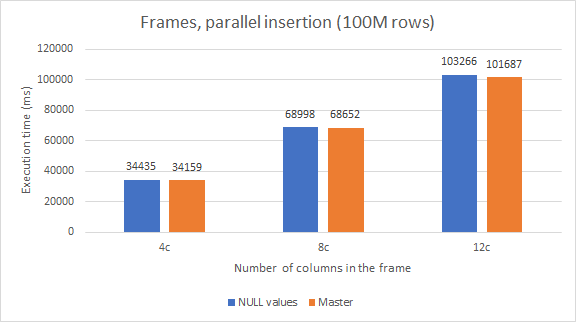
\includegraphics[width=1\textwidth]{chapitre4/Figures/BenchmarkPrallel.png}
  \caption{Benchmark, comparaison entre le temps d'insertion de 100 millions de lignes dans un frame avec et sans support des propriétes NULL}
\end{figure}

\begin{figure}[H]  
  \centering
    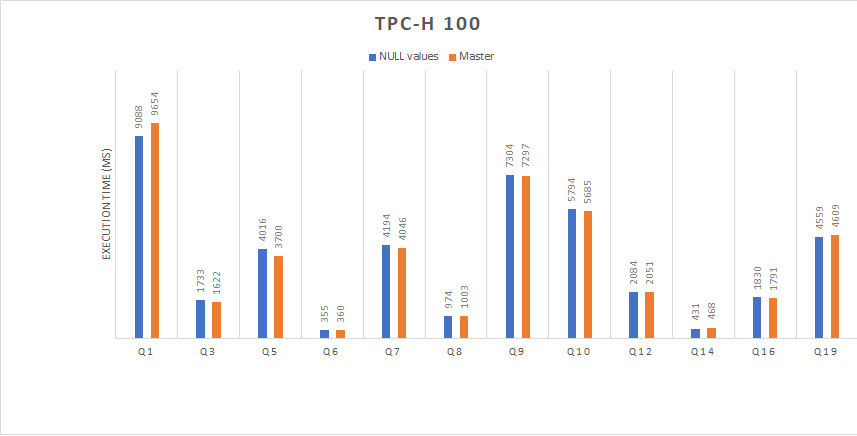
\includegraphics[width=1.1\textwidth]{chapitre4/Figures/BenchmarkTPCH.png}
  \caption{Benchmark TPC-H avec et sans support des propriétes NULL}
\end{figure}

\begin{figure}[H]  
  \centering
    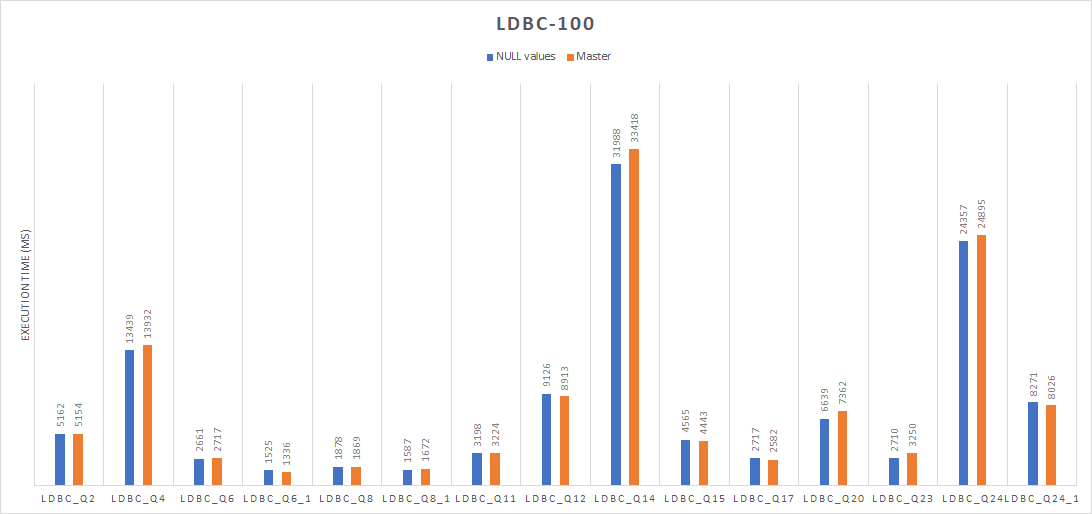
\includegraphics[width=1.1\textwidth]{chapitre4/Figures/BenchmarkLDBC.png}
  \caption{Benchmark LDBC avec et sans support des propriétes NULL}
\end{figure}

\newpage
\section{Conclusion}
Après des évaluations par les pairs et le benchmarking que j’ai réalisé, la conception à étais validé par les membres de l’équipe puisqu’il n’introduit pas un problème de performance considérable.
\begin{itemize}[label=\textbullet]
\item  En mémoire mes modifications on introduit ; 14Mo en mémoire pour un frame de 4 colonnes et 100 millions de rangs.
\item  En matière de temps, les graphiques dans la section précédente montre que mes modifications en introduit une latence négligeable.
\end{itemize}


\chapter{Mise en oeuvre}
Ce chapitre se divise en trois parties, une première partie qui contient la description des différents composants de l’environnement de travail, à savoir les outils de développement utilisés, une deuxième partie où le travail réalisé dans le cadre de ce projet de fin d’études est présenté et une troisième partie qui décrit le travail réalisé et le reste à faire.
\section{Outils de développement}
Cette partie est réservée aux différents outils de travail utilisés durant les différentes phases du projet.

\begin{figure}[h!]  
 \centering
    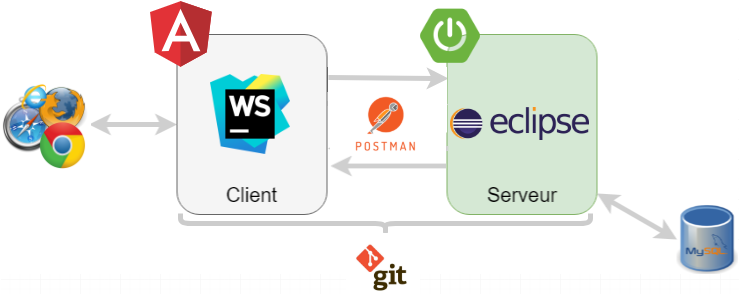
\includegraphics[width=1\textwidth]{chapitre5/Figures/outils.png}
  \caption{Outils utilisés}
\end{figure}

La liste non exhaustive suivante donne une idée sur notre environnement de travail :
\begin{itemize}[label=\textbullet]
  \item Astah permettant la modélisation UML
  \item Eclipse est l'IDE utilisé pour développer le Back-end
  \item Git est le logiciel consacré à la gestion du code source
  \item MySQL a pour but la sauvegarde et la restitution des données
  \item Postman est l'outil choisi pour tester les API REST
  \item WebStorm est l'IDE utilisé pour développer le Front-end
\end{itemize}

Les outils susmentionnés sont décrits en détails dans l'Annexe C.
\section{Réalisation}
L’objectif de cette partie est de donner un aperçu sur les différentes interfaces (IHMs) du système développé, ainsi que les fonctionnalités offertes à l’utilisateur.

\begin{itemize}[label=\textbullet]
%authentification
\item \textbf{Authentification}
Pour accéder aux différentes fonctionnalités de la plateforme, l’utilisateur doit s’authentifier (Figure 5.2)
\begin{figure}[h!]  
 \centering
    
\includegraphics[width=1\textwidth]{chapitre5/Figures/cnx.png}
  \caption{Page d’authentification}
\end{figure}

\begin{itemize}
\item Si les informations entrées par l’utilisateur ne sont pas valides, un message d’avertissement s’affiche (Figure 5.3)
\end{itemize}
\newpage
\begin{figure}[h!]  
 \centering
    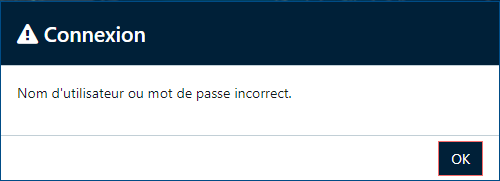
\includegraphics[width=0.7\textwidth]{chapitre5/Figures/errorcnx.png}
  \caption{Message d'avertissement}
\end{figure}

\begin{itemize}
\item Si l’utilisateur oublie son mot de passe, un mail sera envoyé à sa boîte mail (Figure 5.4)
\end{itemize}
\begin{figure}[h!]  
 \centering
    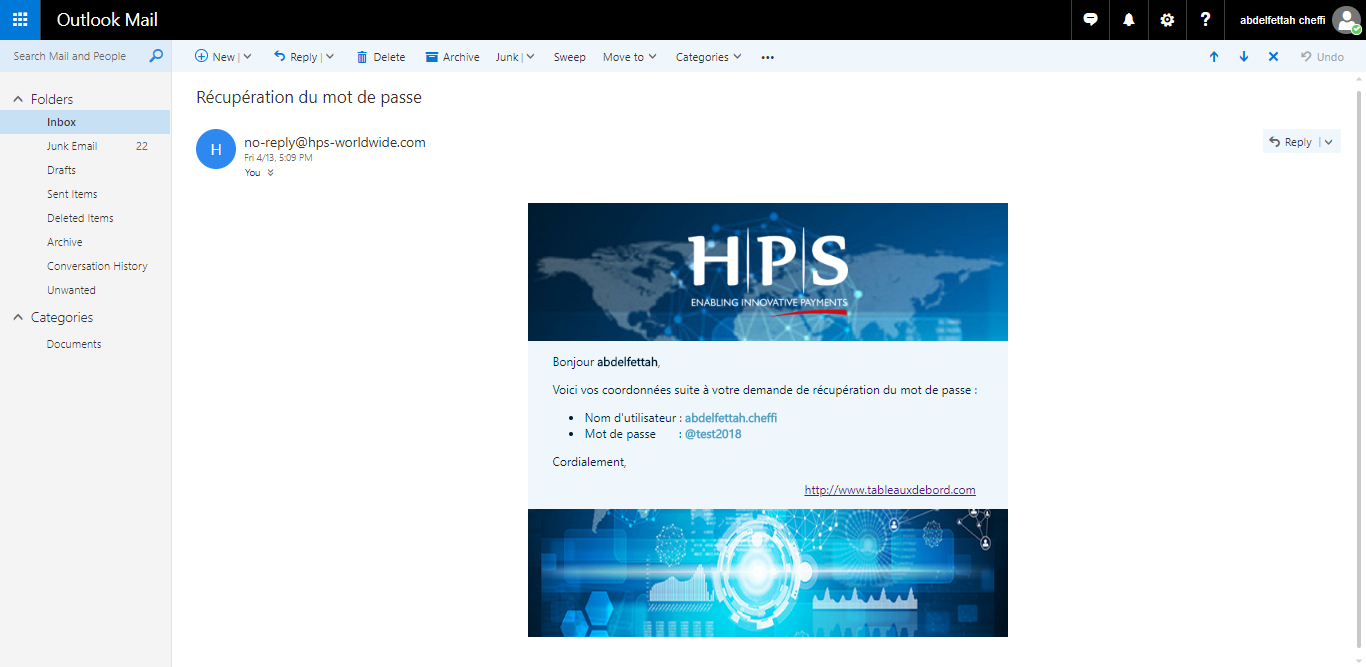
\includegraphics[width=1\textwidth]{chapitre5/Figures/mdpoublie.png}
  \caption{Mail de récupération du mot de passe}
\end{figure}

\begin{itemize}
\item Si la connexion est réussite alors l’utilisateur sera redirigé vers la page d’accueil (Figure 5.5) où il pourra consulter l’application selon son rôle et les droits d’accès qui lui sont attribués 
\end{itemize}
\newpage
\begin{figure}[h!]  
 \centering
    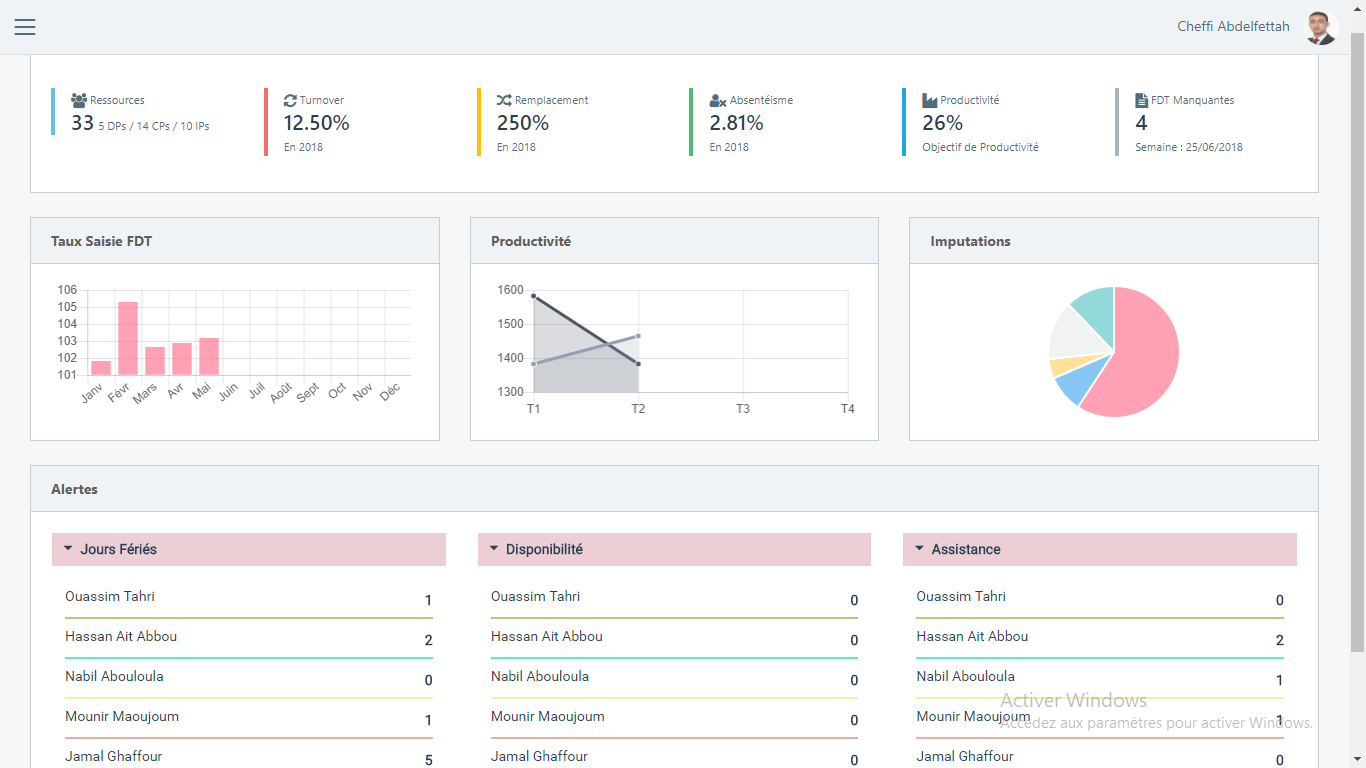
\includegraphics[width=1\textwidth]{chapitre5/Figures/acceuil.png}
  \caption{Page d'accueil}
\end{figure}

\end{itemize}

Cette interface est composée des widgets généraux (nombre ressources, remplacement, absentéisme, FDT manquantes, ...), des graphes (Taux de sasie des FDT, productivité, imputations) ainsi que des alertes.\\
%parametrage
\begin{itemize}[label=\textbullet]
	\item \textbf{Module de paramétrage}
	Ce module permet à l'utilisateur (administrateur et sous-administrateur) de définir les paramètres de l’application.

	\begin{itemize}[label=\textbullet]
	\item Partie administration : cette partie offre les fonctionnalités d'ajout, modification, recherche et suppression et se compose de 4 volets généraux:
	\begin{itemize}
	\item Gestion des agences 
      	\item Gestion des utilisateurs 
     	 \item Gestion des profils 
      	\item Gestion des compétences 
	\end{itemize}
	\end{itemize}
	\newpage
%gestion agence
	\subsubsection*{Exemple "gestion des agences" : }
	\begin{itemize}
			\item Ajouter agence :  l'utilisateur doit respecter la validation correcte des champs des formulaires.
			\begin{figure}[h!]  
			\centering
			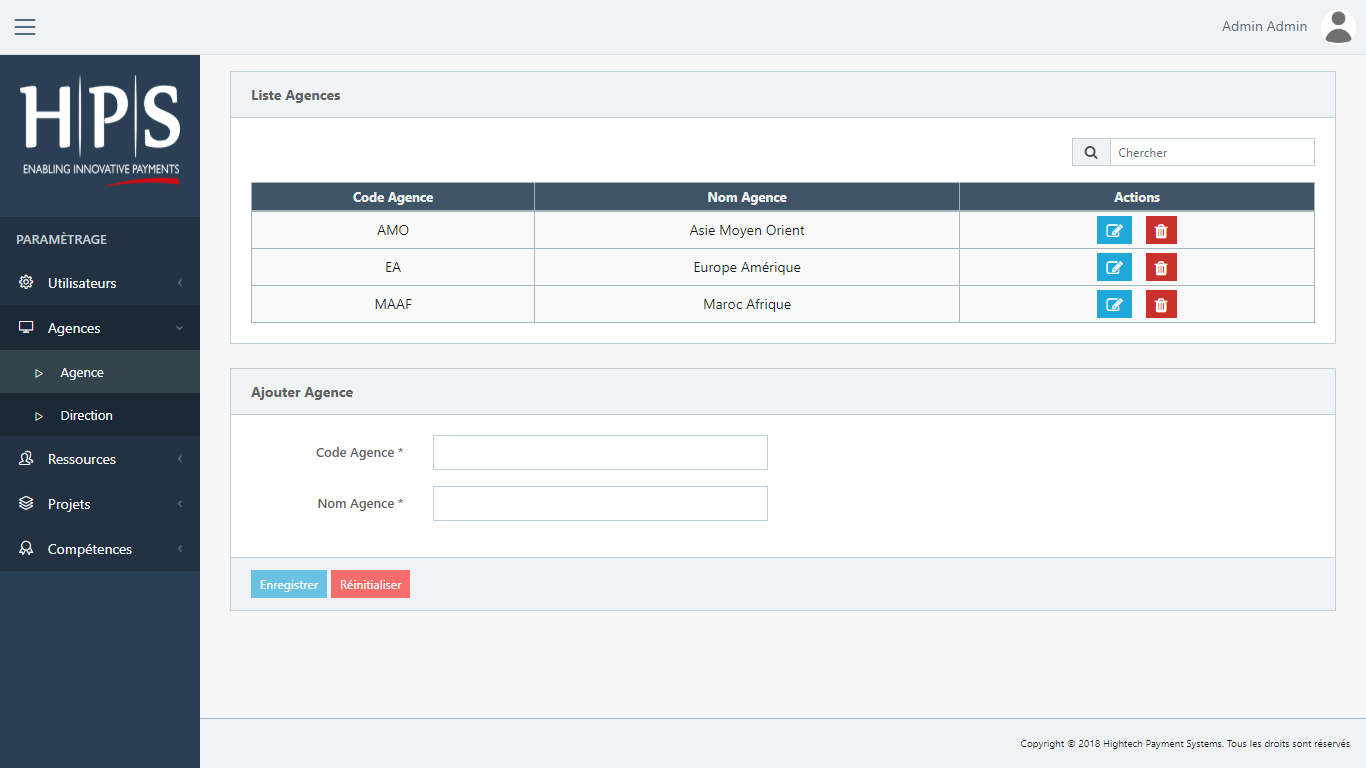
\includegraphics[width=0.9\textwidth]{chapitre5/Figures/addagence.png}
			\caption{Ajouter agence}
			\end{figure}
			\item Supprimer agence : l'utilisateur peut supprimer une agence en cliquant sur le bouton rouge qui correspond à l'enregistrement à supprimer. Un message de confirmation sera affiché
			\begin{figure}[h!]  
			\centering
			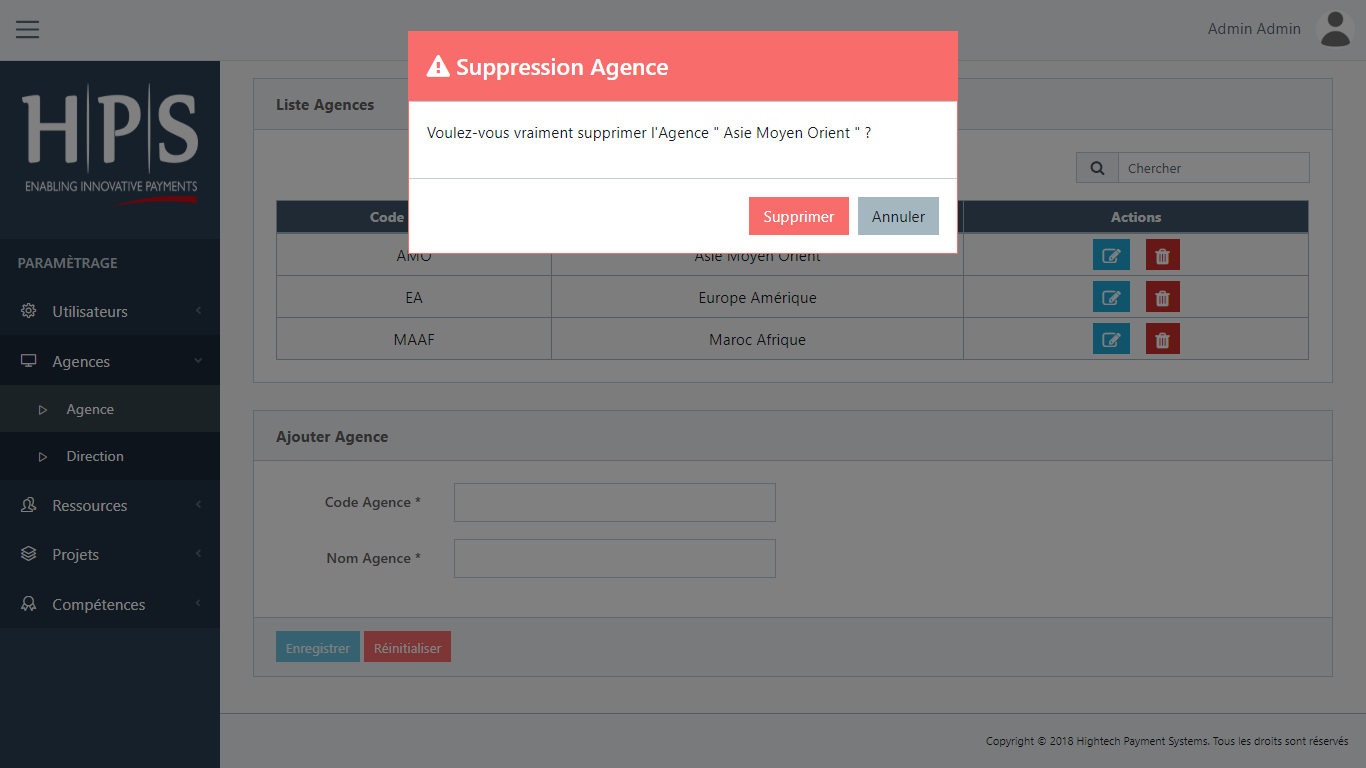
\includegraphics[width=0.9\textwidth]{chapitre5/Figures/supagence.png}
			\caption{Supprimer agence}
			\end{figure}
\newpage
			\item Modifier agence : l'utilisateur choisit un enregistrement à modifier, en cliquant dessus il sera redirigé à l'interface suivante
			\begin{figure}[h!]  
			\centering
			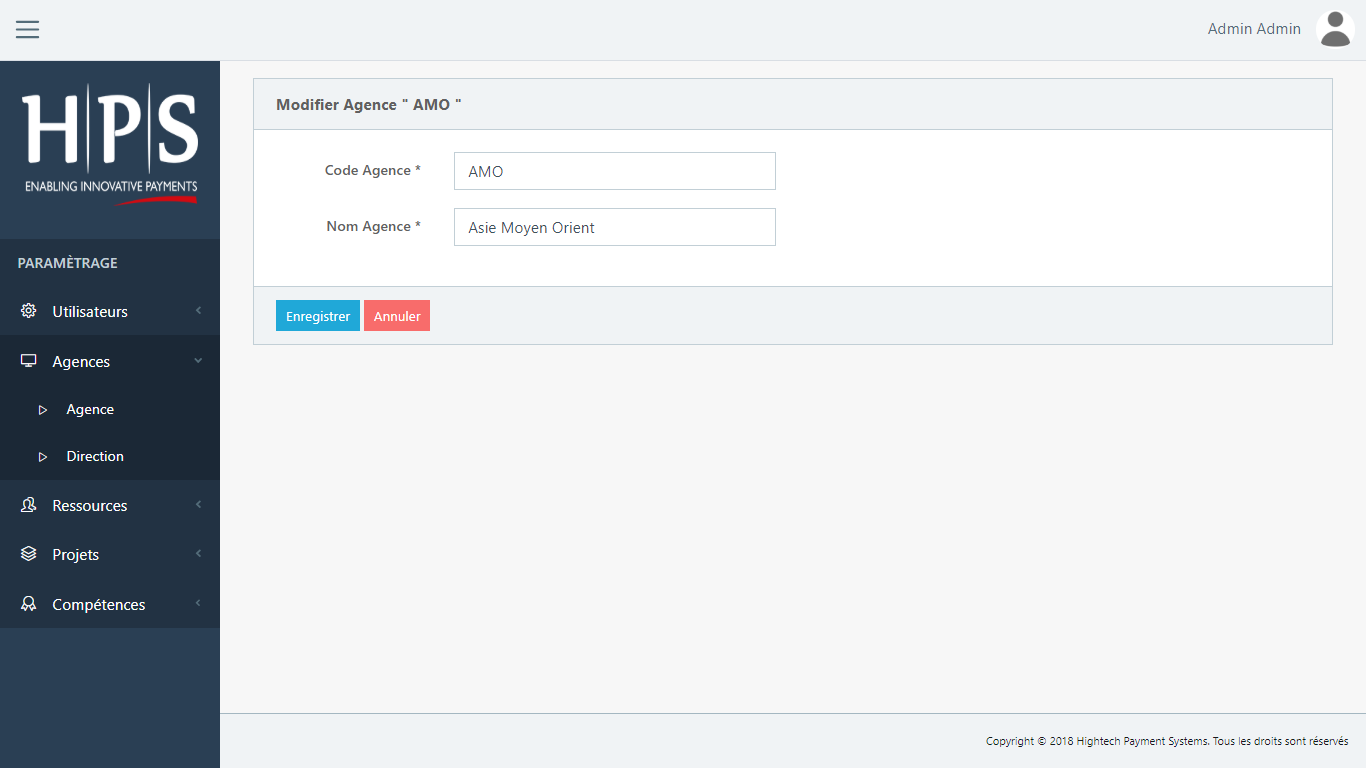
\includegraphics[width=1\textwidth]{chapitre5/Figures/modagence.png}
			\caption{Modifier agence}
			\end{figure}
			\end{itemize}

\begin{itemize}[label=\textbullet]
		\item Partie sous-administration : cette partie offre les fonctionnalités d’ajout, modification, recherche et suppression et se compose de 4 volets relatifs à l'agence de l'utilisateur connecté :
		\begin{itemize}
		\item Gestion des clients
      		\item Gestion des ressources
      		\item Gestion des pays et régions
      		\item Gestion des droits d'accès
		\end{itemize}
	\end{itemize}

%gestion ressource
\subsubsection*{Exemple "gestion des ressources" : }
\begin{itemize}
			\item Ajouter ressource projet :  l'utilisateur doit respecter la validation correcte des champs des formulaires.  \newpage
			\begin{figure}[h!]  
			\centering
			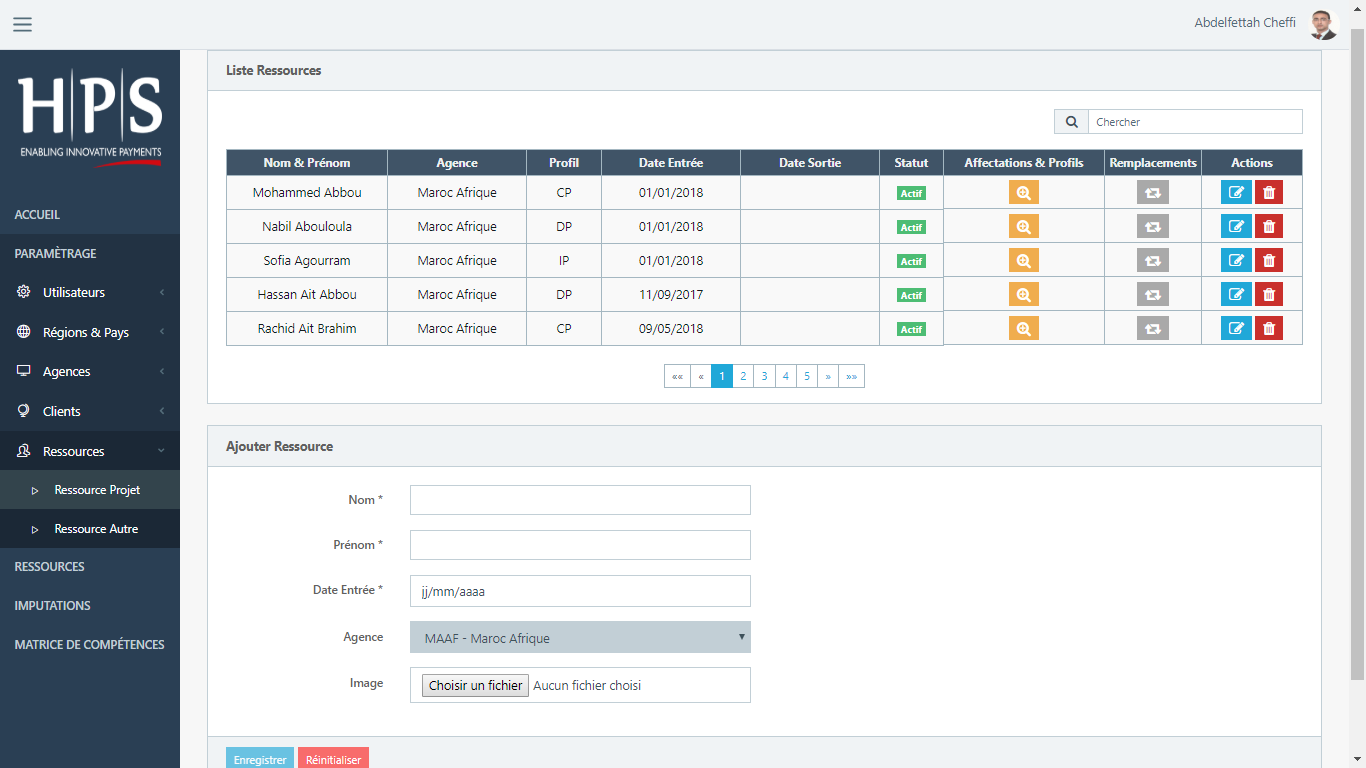
\includegraphics[width=1\textwidth]{chapitre5/Figures/addressource.png}
			\caption{Ajouter ressource projet}
			\end{figure}
			\item Supprimer ressouce projet : l'utilisateur peut supprimer une ressource projet en cliquant sur le bouton rouge qui correspond à l'enregistrement à supprimer. Un message de confirmation sera affiché
			\begin{figure}[h!]  
			\centering
			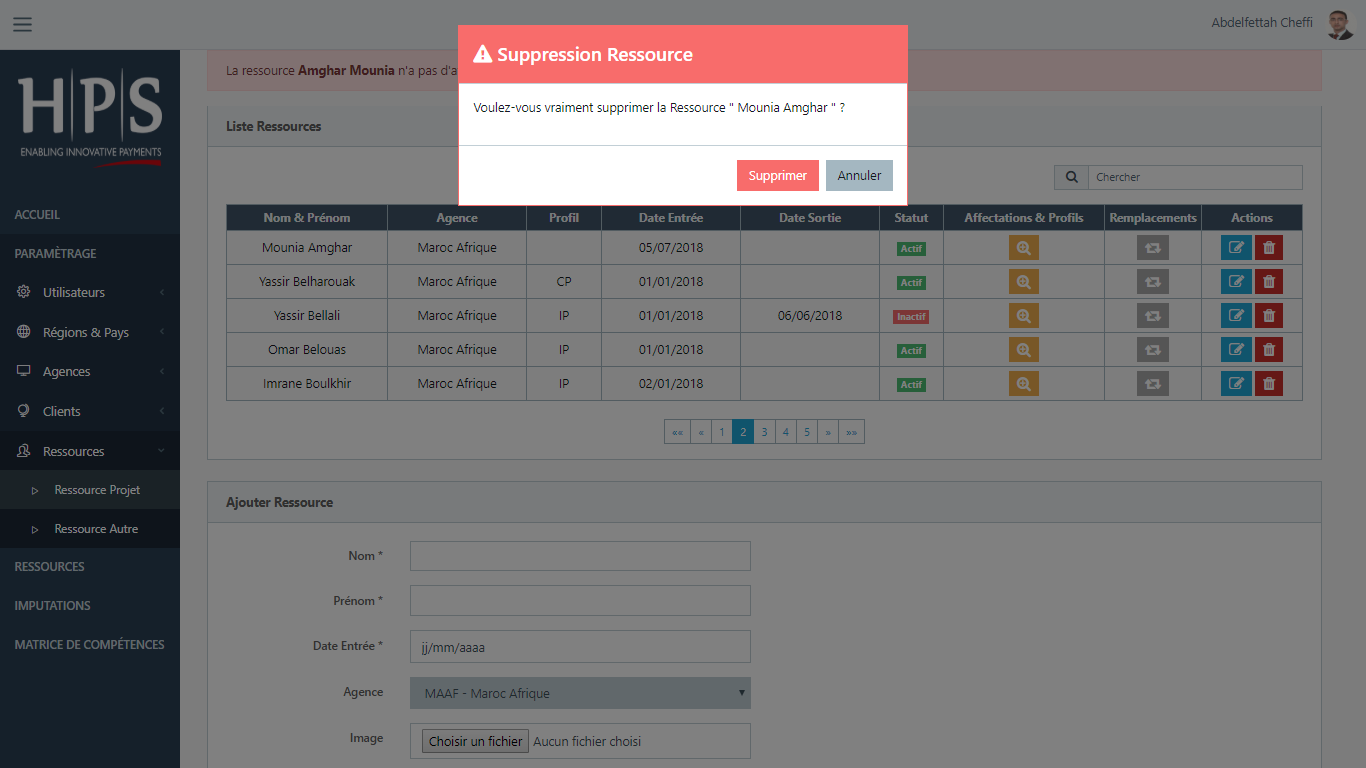
\includegraphics[width=1\textwidth]{chapitre5/Figures/supressource.png}
			\caption{Supprimer ressource projet}
			\end{figure}
			\item Modifier ressouce projet : l'utilisateur choisit un enregistrement à modifier, en cliquant dessus il sera redirigé à l'interface suivante
			\begin{figure}[h!]  
			\centering
			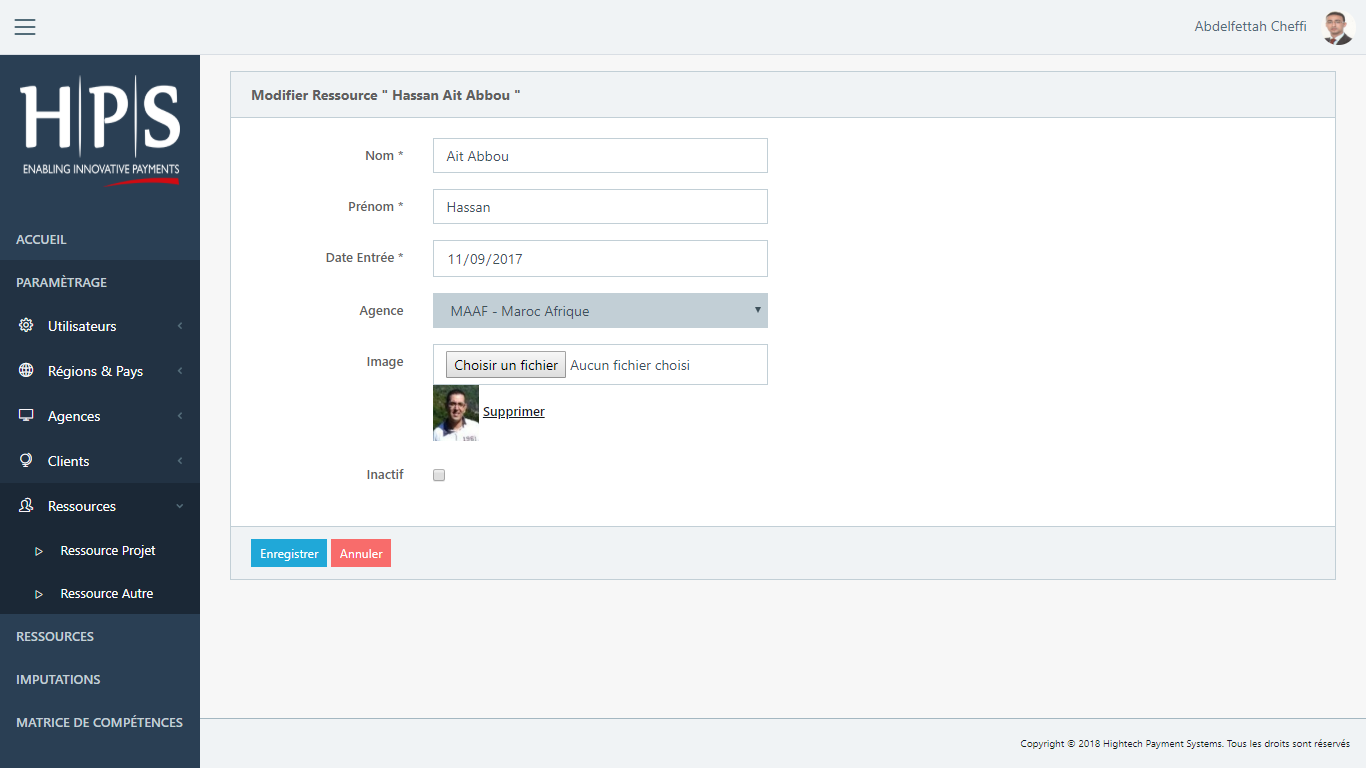
\includegraphics[width=1\textwidth]{chapitre5/Figures/modressource.png}
			\caption{Modifier ressource projet}
			\end{figure}
			\item Remplacer ressource projet : l'utilisateur choisit une ressource à remplacer, en cliquant sur le bouton correspondant il sera redirigé à l'interface suivante où il pourra choisir la ressource qui va la remplacer
			\begin{figure}[h!]  
			\centering
			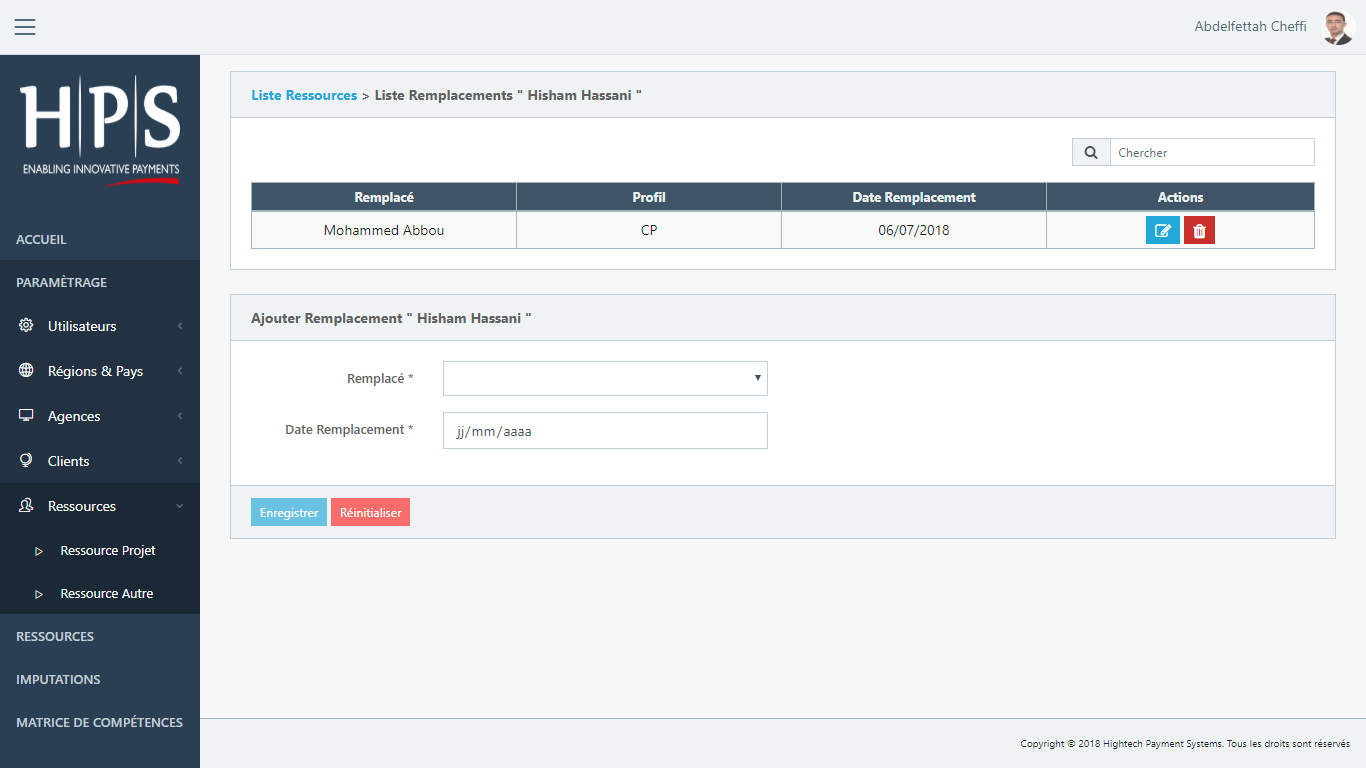
\includegraphics[width=1\textwidth]{chapitre5/Figures/rempressource.png}
			\caption{Remplacer ressource projet}
			\end{figure}
			\item Affecter ressource projet : quand une ressource est ajoutée, elle n'as pas de profil, par suite il faut ajouter une affectation à la ressource. Une affectation pourra être ajouter, modifier ou supprimer
			\begin{figure}[h!]  
			\centering
			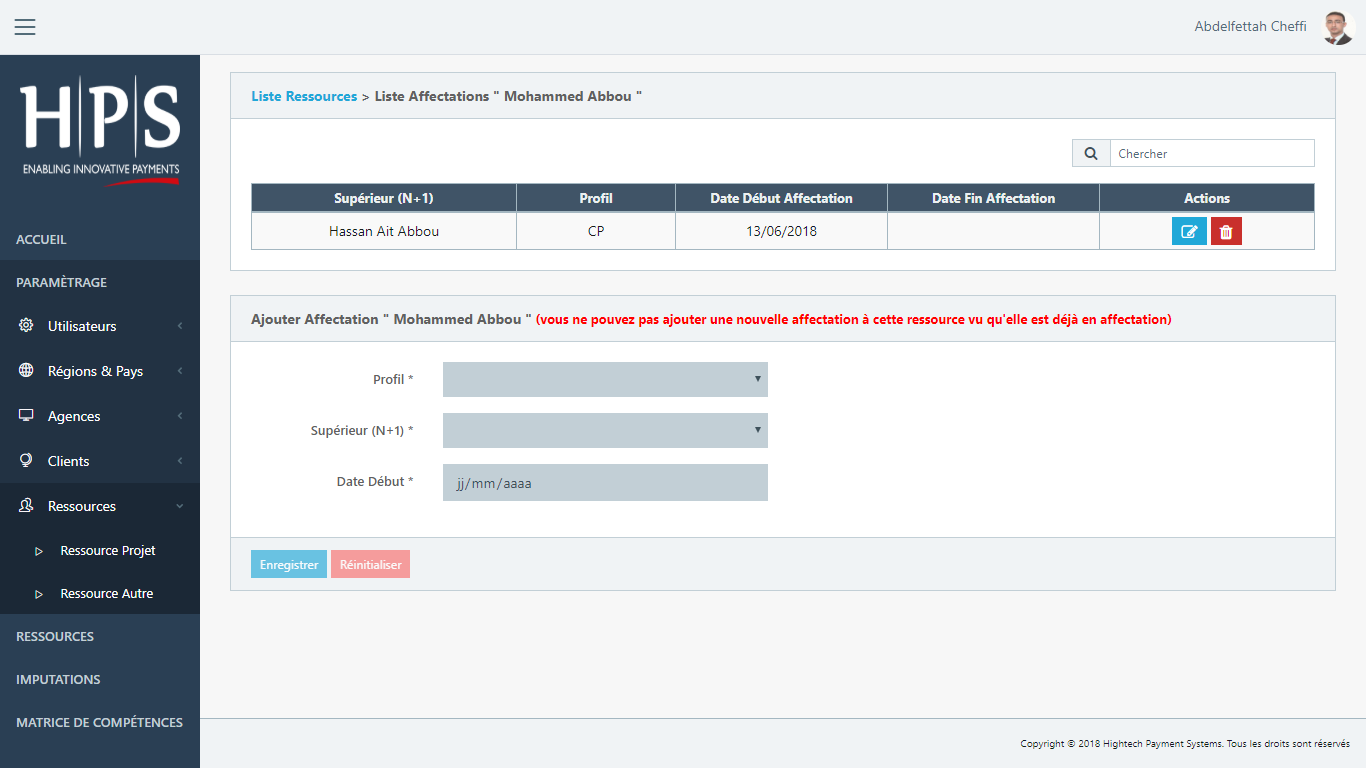
\includegraphics[width=1\textwidth]{chapitre5/Figures/affressource.png}
			\caption{Affecter ressource projet}
			\end{figure}
			\end{itemize}
%gestion des droit d'accées
\subsubsection*{Exemple "gestion des droits d'accès" : }
Cette interface permet au sous-administrateur d'attribuer les droits d'accès d'une rubrique à un profil
\begin{figure}[h!]  
			\centering
			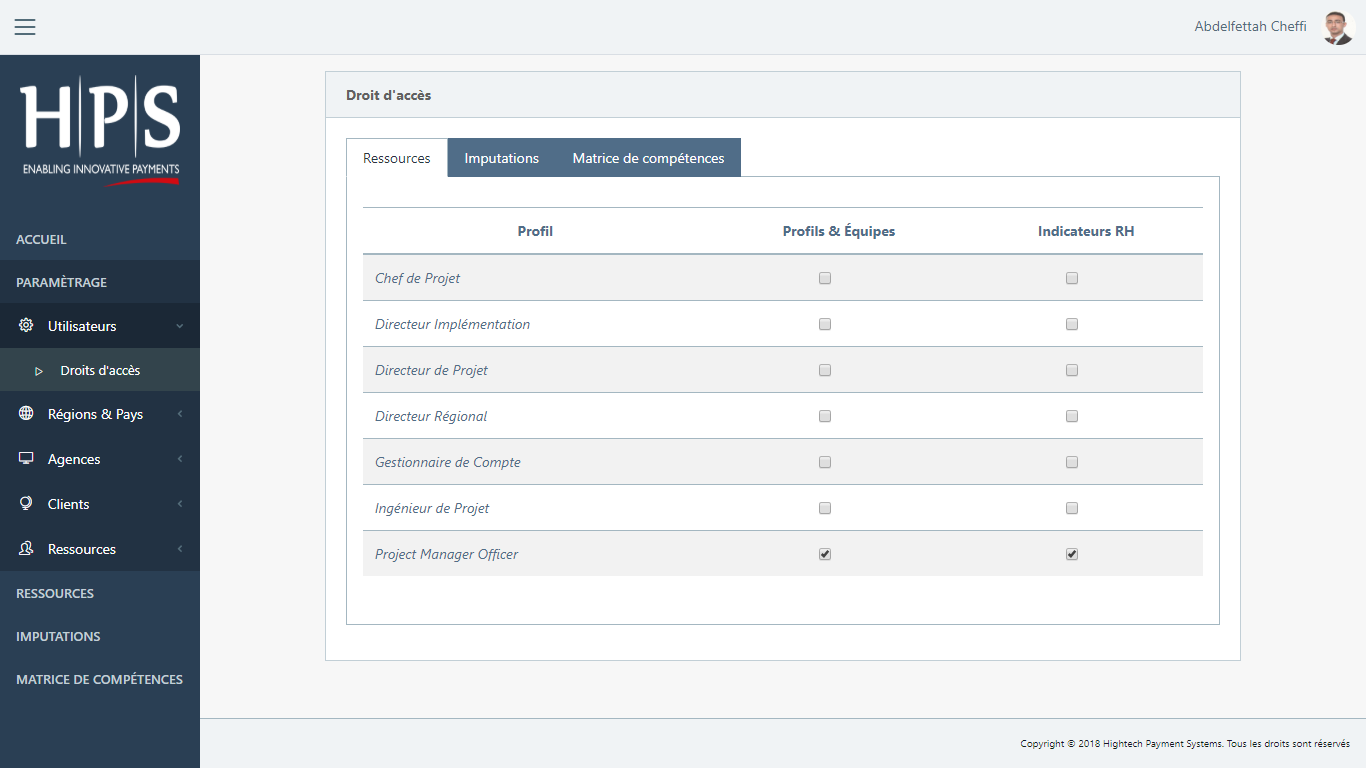
\includegraphics[width=1\textwidth]{chapitre5/Figures/droit.png}
			\caption{Droits d'accès}
			\end{figure}


%%%%module resspources
\item \textbf{Module de suivi des ressources}
	Ce module permet aux collaborateurs le suivi des resssources.
\begin{itemize}
\item \textbf{Profils et équipes }
\begin{figure}[h!]  
			\centering
			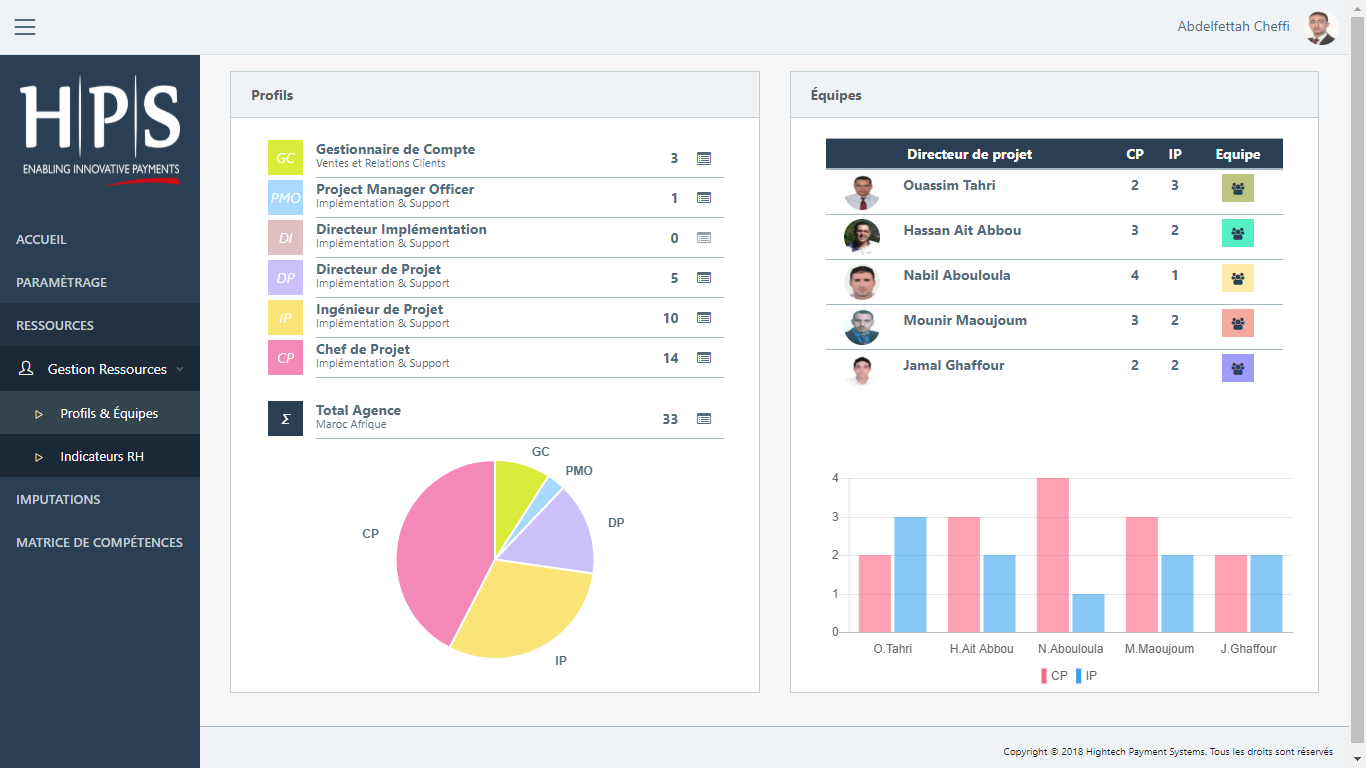
\includegraphics[width=1\textwidth]{chapitre5/Figures/proequ.png}
			\caption{Profils et équipes}
			\end{figure}
\\
Cette interface permet à l'utilisateur de consulter le nombre de ressources et leurs noms par profil (Figure 5.16) ainsi que les équipes de chaque directeur de projet (Figure 5.17).
\begin{figure}[h]
    \begin{minipage}[c]{.46\linewidth}
        \centering
        \includegraphics[width=1\textwidth]{chapitre5/Figures/profil.png}
        \caption{Ressources par profil}
    \end{minipage}
    \hfill%
    \begin{minipage}[c]{.46\linewidth}
        \centering
        \includegraphics[width=1\textwidth]{chapitre5/Figures/equipes.png}
        \caption{Equipes par DP}
    \end{minipage}
\end{figure}
\newpage
\item \textbf{Indicateurs RH }
\begin{figure}[h!]  
			\centering
			\includegraphics[width=1\textwidth]{chapitre5/Figures/indicateur.png}
			\caption{Indicateurs RH}
			\end{figure}
\\
  Cette interface représente le nombre des départs et d'entrées ainsi que le taux de remplacement, turnover et absentéisme dans l'agence.\\
Pour chaque indicateur, on peut avoir les détails (Figure 5.19)
\begin{figure}[h!]  
			\centering
			\includegraphics[width=0.8\textwidth]{chapitre5/Figures/details.png}
			\caption{Détails de l'indicateur absentéisme}
			\end{figure}
\end{itemize}
%%%suivi imputation
\item \textbf{Module de suivi des imputations}
	Ce module permet aux collaborateurs de représenter les statistiques liées à la saisie des feuilles de temps des ressources.
\begin{itemize}
\item \textbf{Suivi des FDT}
\begin{figure}[h!]  
			\centering
			\includegraphics[width=1\textwidth]{chapitre5/Figures/fdt.png}
			\caption{Suivi des FDT}
			\end{figure}
\\
Cette interface se divise en deux parties, la première permet l'affichage des FDT manquantes et le taux de saisie par directeur de projet et par agence pour chaque semaine ainsi que la saisie des FDT manquantes (Figure 5.21). La deuxième affiche l'évolution hebdomadaire du taux de saisie et FDT manquantes par agence et par directeur de projet (Figure 5.22)
\begin{figure}[h]
    \begin{minipage}[c]{.46\linewidth}
        \centering
        \includegraphics[width=0.97\textwidth]{chapitre5/Figures/saisiefdt.png}
        \caption{Ressources par profil}
    \end{minipage}
    \hfill%
    \begin{minipage}[c]{.46\linewidth}
        \centering
        \includegraphics[width=1\textwidth]{chapitre5/Figures/evolution.png}
        \caption{évolution hebdomadaire du taux de saisie par directeur de projet}
    \end{minipage}
\end{figure}
\newpage
\item \textbf{Taux de Saisie}
\begin{figure}[h!]  
			\centering
			\includegraphics[width=0.92\textwidth]{chapitre5/Figures/taux.png}
			\caption{Taux de Saisie}
			\end{figure}
\\
Cette interface représente le taux de saisie des FDT mensuellement de l'agence.
\end{itemize}
%%matrice des competence
\item \textbf{Module de la matrice de compétences}
Ce module permet d’évaluer les compétences des ressources et de connaitre réellement leurs niveaux sur plusieurs domaines.
\begin{itemize}
\item \textbf{Evaluation}
\begin{figure}[h!]  
			\centering
			\includegraphics[width=0.92\textwidth]{chapitre5/Figures/evaluation.png}
			\caption{Evaluation}
			\end{figure}
\newpage
Cette interface permet au directeur de projet d'évaluer les compétences de ces ressources.
\item \textbf{Synthèse}
\begin{figure}[h!]  
			\centering
			\includegraphics[width=1\textwidth]{chapitre5/Figures/synthese.png}
			\caption{Synthèse}
			\end{figure}
\\
Cette interface permet d'afficher des graphes syntétisant l'évaluation des resources selon des critères définis par l'utilisateur.
\end{itemize}
\end{itemize}
\section{Travail réalisé et reste à faire}
L'ensemble du projet contient 5 modules (paramétrage, suivi des ressources, suivi des imputations, la matrice des compétences et suivi des projets), on a réalisé les modules paramétrage, suivi des ressources, une partie de suivi des imputations ( les FDT) et la matrice des compétences. La partie restante du module suivi des imputations (Productivité) et le module suivi des projets restent à développer.
\newpage
\begin{figure}[h!]  
	\centering
	\includegraphics[width=1\textwidth]{chapitre5/Figures/avancement.png}
	\caption{Pourcentage d'avancement par rapport au cahier de charge}
\end{figure}
\section*{Conclusion}
Ce dernier chapitre a servi à introduire les outils de développement utilisés afin de présenter par la suite le travail réalisé pour concrétiser le travail mené dans l’étude fonctionnelle ainsi que le reste à faire.
\chapter*{Conclusion générale et perspectives}
\addcontentsline{toc}{chapter}{Conclusion Générale}
Notre projet de fin d’études effectué au sein de HPS consiste à concevoir et réaliser une application d’automatisation des tableaux de bord et indicateurs. Cette solution a pour but de faciliter, standardiser et optimiser la génération des tableaux de bord pour l’ensemble des parties prenantes.\\ \\
Afin de réaliser ces objectifs, il s’est avéré primordial de recenser les besoins fonctionnels et techniques de l’application. Cette étape nous a permis de passer à la conception de la solution en se basant sur le formalisme UML. Et enfin la bonne gestion de la phase de réalisation, en respectant les principes de la méthodologie agile SCRUM, nous ont permis d’implémenter, tester et valider les différentes évolutions réalisées conformément aux spécifications et respectant les contraintes projet défini dans le plan qualité projet.\\ \\
En guise de perspectives : 
\begin{itemize}[label=\textbullet]
\item On envisage d'offrir à l'utilisateur la possibilité d'extraire les différentes informations sous forme excel afin de les exploiter
\item Interfaçage entre project server et l'application afin de récuperer les données en temps réel sans attendre la fin de chaque mois.
\end{itemize}
\renewcommand\appendixname{Annexes}
  \renewcommand\appendixpagename{Annexes}
\renewcommand\appendixtocname{Annexes}
\begin{appendices}
    \chapter{Méthodes agiles}
Une méthode agile est une approche itérative et incrémentale, qui est menée dans un esprit collaboratif avec juste ce qu’il faut de formalisme.\\
Elle génère un produit de haute qualité tout en prenant en compte l’évolution des besoins des clients. Il existe plusieurs méthodes : Scrum (la plus populaire), XP, le lean software développement, etc. et les techniques proposées sont nombreuses.

\section{Valeurs caractéristiques d’un projet agile}
\begin{itemize}[label=\textbullet]
\item Les individus et les interactions plutôt que les processus et les outils
\item Produit qui fonctionne plutôt qu’une documentation exhaustive
\item La collaboration avec le client plutôt que la contractualisation des relations
\item L’acceptation du changement plutôt que la conformité aux plans
\end{itemize}

\section{Les douzes principes d’une méthode agile}
\begin{itemize}[label=\textbullet]
\item Satisfaire le client est la priorité
\item Accueillir les demandes de changement « à bras ouverts »
\item Livrer le plus souvent possible des versions opérationnelles de l’application
\item Assurer une coopération permanente entre Client et Equipe projet
\item Construire des projets autour d’individus motivés
\item Privilégier la conversation en face à face
\item Mesurer l’avancement du projet en termes de fonctionnalités de l’application
\item Faire avancer le projet à un rythme soutenable et constant
\item Porter une attention continue à l’excellence technique et à la conception
\item Favoriser la simplicité
\item Responsabiliser les équipes
\item Ajuster, à intervalles réguliers, son comportement, ses processus pour être plus efficace
\end{itemize}

\section{L’agilité avec Scrum}
Scrum est un processus agile qui nous conduit à produire la plus grande valeur métier dans la durée la plus courte.\\
Scrum nous permet d’inspecter rapidement et régulièrement (toutes les 1 à 4semaines) un produit
(partiel) qui fonctionne.\\
Le métier identifie les exigences et définit leur priorité. Notre équipe s’organise elle-même pour déterminer
la meilleure façon de produire les exigences les plus prioritaires.
\begin{figure}[h!]  
 \centering
    \includegraphics{annexe/Figures/scrum.png}
  \caption{Cycle de vie de la méthode SCRUM}
\end{figure}

Toutes les 1 à 4 semaines, tout le monde peut voir fonctionner le produit actuel et contribuer
à prendre une décision : soit le livrer dans l’état, soit continuer à l’améliorer pendant 2 à 4 semaines
supplémentaires avant de se reposer la question.\\

\subsubsection*{Release}
Pour améliorer la lisibilité du projet, on regroupe généralement des itérations en releases.
Bien que ce concept ne fasse pas explicitement partie de Scrum, il est utilisé pour mieux identifier
les versions. En effet, comme chaque sprint doit aboutir à la livraison d’un produit partiel, un release
permet de marquer la livraison d’une version aboutie, susceptible d’être mise en exploitation.
Il est intéressant de planifier à l’échelle d’un release, en répartissant les items du backlog de produit
sur les sprints, en respectant leur priorité. Bien entendu, ce qui est planifié au-delà du sprint courant
peut changer à tout moment, rien n’est figé à l’avance.\\
\subsubsection*{Sprints}
À la fin du sprint, tout le monde se réunit pour effectuer la revue de sprint, qui dure au maximum 4
heures. L’objectif de la revue de sprint est de valider le logiciel qui a été produit pendant le sprint.
L’équipe commence par énoncer les items du backlog de produit qu’elle a réalisés. Elle effectue ensuite
une démonstration du logiciel produit. C’est sur la base de cette démonstration que le directeur
de produit valide chaque fonctionnalité planifiée pour ce sprint.\\
Une fois le bilan du sprint réalisé, l’équipe et le directeur de produit proposent des aménagements sur
le backlog du produit et sur la planification provisoire de la release. Il est probable qu’à ce moment
des items soient ajoutés, modifiés ou ré-estimés, en conséquence de ce qui a été découvert.
    \chapter{REST API}
\begin{figure}[h!]  
 \centering
    \includegraphics[width=0.6\textwidth]{annexe/Figures/rest.png}
\end{figure}
REST, acronyme de Representational State Transfer, est un style d’architecture logiciel qui définit la communication entre les différentes parties du web. L’échange est basé sur des requêtes client et serveur. Un client interroge le serveur par une requête HTTP, et le serveur renvoie une réponse. Cette interrogation se fait suivant différentes méthodes : 
\begin{itemize}[label=\textbullet]
\item GET pour la lecture des données
\item POST pour les créer
\item PUT pour les mettre à jour 
\item DELETE pour les supprimer
\end{itemize}

REST n’impose pas un format d’échange entre le client et le serveur. La réponse envoyée par le serveur peut avoir plusieurs présentations : HTML, XML, JSON, .... C’est au développeur de définir quel format pour la représentation de réponse le convient le mieux
\end{appendices}
\chapter*{Références}
\textbf{\underline{a. Bibliographie :}} 
\begin{enumerate}[label={[\arabic*]}]

\item Calvin Lin, Larry Snyder \textit{Principles of Parallel Programming} -Pearson : 2008
\item Nicholas P. Roth, Vasileios Trigonakis, Sungpack Hong, Hassan Chafi, Anthony Potter, BorisMotik, and Ian Horrocks \textit{Pgx.d/async: A scalable distributed graph pattern matching engine} - In Proceedings of the Fifth International Workshop on Graph Data-management Experiences \& Systems, GRADES’17, pages 7:1–7:6, : New York, NY, USA, 2017. ACM.
\item S. Hong, S. Depner, T.Manhardt, J. Van Der Lugt, M. Verstraaten, and H. Chafi. \textit{Pgx.d: a fast distributed graph processing engine } In SC ’15: Proceedings of the International Conference for High Performance Computing, Networking, Storage and Analysis, pages 1–12, : Nov 2015
\item Vasileios Trigonakis, Damien Hilloulin \textit{EPFL-On-Campus-2019.pptx} - présentation de PGX aux étudiants d’EPFL : 2019
\item D. Easley and J. Kleinberg \textit{Networks, crowds, and markets: Reasoning about a highly connected world} - Cambridge University Press : 2010
\end{enumerate}\\


\textbf{ \underline{b. Webographie :} } 
\begin{enumerate}[label={[\arabic*]}]
\item{Cplusplus.com, http://www.cplusplus.com/reference/bitset/bitset/}
\item{Neo4j https://neo4j.com/developer/ : 2017}
\item{Oracle big data, https://medium.com/oracledevs/5-innovative-ways-to-use-graph-analytics-bacc4f2be521, Medium : 2018}
\item{Oskar van Rest, Sungpack Hong, Jinha Kim, Xuming Meng, and Hassan Chafi \textit{PGQL Specifications} http://pgql-lang.org/spec/1.3/ : 2020.}
\item{TPC.org, http://www.tpc.org/tpch/default5.asp}
\item{Wikipedia, https://en.wikipedia.org/wiki/Sun\_Microsystems}
\item{labs.oracle.com, https://labs.oracle.com/pls/apex/f?p=94065:INTRO::::::}
\item{https://en.wikipedia.org/wiki/Connectivity\_(graph\_theory)}
\item{https://www.coursera.org/lecture/cloud-computing-2/distributed-graph-processing-TTdWS}
\item{https://en.wikipedia.org/wiki/Raft\_(computer\_science)}
\item{https://blog.stackpath.com/distributed-system/}
\item{https://www.gartner.com/en/newsroom/press-releases/2019-02-18-gartner-identifies-top-10-data-and-analytics-technolo}
\item{https://en.wikipedia.org/wiki/Oracle\_Corporation}
\end{enumerate}\\


%\renewcommand
%\part{R\'ef\'erences}
%\newpage
%\addcontentsline{toc}{chapter}{R\'ef\'erences}
%\bibliography
%\chapter{R\'ef\'erences}
%\renewcommand\bibname{Webographie}
%\begin{thebibliography}{20}
%\bibitem hhttps://www.g2crowd.com/compare/
%\bibitem hhttps://www.hps-worldwide.com/
%\bibitem hhttp://www.qualitystreet.fr/2007/11/20/methodes-agiles-un-belle-definition/
%\bibitem hhttp://docs.spring.io/spring-security/site/docs/3.2.4.RELEASE/reference/htmlsingle/
%\bibitem hhttps://blog.davincisoftware.sk/blog-angular-and-spring-security-integration-part1
%\bibitem hhttps://blog.davincisoftware.sk/blog-angular-and-spring-security-integration-part2

%\end{thebibliography}




\printindex
\end{document}
